%%%%%%%%%%%%%%%%%%%%%%%%%%%%%%%%%%%%%%%%%%%%%%%%%%%%%%%%%%%%
% 5.1 PRECALCULUS & FUNCTIONS
% The Composition of Advanced Mathematics
%%%%%%%%%%%%%%%%%%%%%%%%%%%%%%%%%%%%%%%%%%%%%%%%%%%%%%%%%%%%

\section{Precalculus and Functions}
\label{sec:precalculus-functions}

\prerequisite{
Arithmetic foundations from \cref{sec:arithmetic-foundations}, number
systems from \cref{sec:number-systems}, elementary set theory from
\cref{sec:elementary-set-theory}, relations from \cref{sec:relations},
functions from \cref{sec:functions}, and elementary algebra from
\cref{sec:elementary-algebra}.
}

\learningobjectives{
By the end of this section, the reader should be able to:
\begin{itemize}
    \item interpret functions numerically, algebraically, graphically, and verbally;
    \item determine domains, ranges, intercepts, zeros, and intervals of behavior;
    \item evaluate and manipulate functions using function notation;
    \item recognize and analyze polynomial, rational, radical, absolute-value,
    exponential, logarithmic, trigonometric, and piecewise-defined functions;
    \item construct new functions through transformations, arithmetic operations,
    composition, and inversion;
    \item distinguish even, odd, periodic, increasing, decreasing, and bounded behavior;
    \item determine average rates of change and interpret secant slopes;
    \item work with exponential and logarithmic models;
    \item use radian measure and the unit circle to define trigonometric functions;
    \item understand inverse trigonometric functions and their restricted domains;
    \item identify asymptotic behavior;
    \item connect function behavior with the ideas of limits and calculus.
\end{itemize}
}

%%%%%%%%%%%%%%%%%%%%%%%%%%%%%%%%%%%%%%%%%%%%%%%%%%%%%%%%%%%%
\subsection{Why Precalculus Matters}
\label{subsec:why-precalculus}
%%%%%%%%%%%%%%%%%%%%%%%%%%%%%%%%%%%%%%%%%%%%%%%%%%%%%%%%%%%%

Calculus studies change.

Analysis studies the logical and structural foundations behind limits,
continuity, differentiation, integration, convergence, and related ideas.

Both subjects depend on a strong understanding of functions.

A function may describe:

\begin{itemize}
    \item position as a function of time;
    \item population as a function of year;
    \item temperature as a function of location;
    \item pressure as a function of volume;
    \item revenue as a function of quantity sold;
    \item probability as a function of a parameter;
    \item the solution of a differential equation as a function of time.
\end{itemize}

Precalculus develops the language needed to describe and analyze these
relationships before introducing limiting processes.

\begin{conceptbox}
The central object of calculus and analysis is the \textbf{function}.

Precalculus develops the algebraic, graphical, numerical, and geometric
language required to study how functions behave and how their outputs change.
\end{conceptbox}

%%%%%%%%%%%%%%%%%%%%%%%%%%%%%%%%%%%%%%%%%%%%%%%%%%%%%%%%%%%%
\subsection{Functions Revisited}
\label{subsec:analysis-functions-revisited}
%%%%%%%%%%%%%%%%%%%%%%%%%%%%%%%%%%%%%%%%%%%%%%%%%%%%%%%%%%%%

Recall that a function

\[ f:A\to B \]

assigns exactly one element of \(B\) to each element of \(A\).

The notation is read:

``\(f\) maps \(A\) to \(B\).''

For an input \(x\in A\), the corresponding output is written

\[ f(x). \]

This is read ``\(f\) of \(x\).''

The set \(A\) is the \emph{domain}.

The set \(B\) is the \emph{codomain}.

The set of outputs actually attained by \(f\) is its \emph{range} or image.

%%%%%%%%%%%%%%%%%%%%%%%%%%%%%%%%%%%%%%%%%%%%%%%%%%%%%%%%%%%%
\subsection{Function Notation}
\label{subsec:analysis-function-notation}
%%%%%%%%%%%%%%%%%%%%%%%%%%%%%%%%%%%%%%%%%%%%%%%%%%%%%%%%%%%%

Suppose

\[ f(x)=x^2-3x+4. \]

Then

\[ f(2)=2^2-3(2)+4=2. \]

To evaluate at an expression such as \(x+h\), substitute the entire
expression:

\[
f(x+h)=(x+h)^2-3(x+h)+4.
\]

Expanding,

\[
f(x+h)=x^2+2xh+h^2-3x-3h+4.
\]

This type of substitution becomes especially important when constructing
difference quotients.

%%%%%%%%%%%%%%%%%%%%%%%%%%%%%%%%%%%%%%%%%%%%%%%%%%%%%%%%%%%%
\subsection{Worked Example: Evaluating a Function}
\label{subsec:worked-function-evaluation}
%%%%%%%%%%%%%%%%%%%%%%%%%%%%%%%%%%%%%%%%%%%%%%%%%%%%%%%%%%%%

\begin{workedexamplebox}{Evaluating Function Expressions}

Let

\[ f(x)=2x^2-5x+1. \]

Find \(f(-2)\) and \(f(a+1)\).

\begin{tabularx}{\textwidth}{@{}>{\raggedright\arraybackslash}p{0.42\textwidth}X@{}}
Substitute \(x=-2\). &
\(f(-2)=2(-2)^2-5(-2)+1\)\\
Simplify. &
\(f(-2)=8+10+1=19\)\\[2mm]
Substitute \(x=a+1\). &
\(f(a+1)=2(a+1)^2-5(a+1)+1\)\\
Expand. &
\(f(a+1)=2a^2+4a+2-5a-5+1\)\\
Combine like terms. &
\(f(a+1)=2a^2-a-2\)
\end{tabularx}

\begin{answerbox}
\[ \boxed{f(-2)=19,\qquad f(a+1)=2a^2-a-2.} \]
\end{answerbox}
\end{workedexamplebox}

%%%%%%%%%%%%%%%%%%%%%%%%%%%%%%%%%%%%%%%%%%%%%%%%%%%%%%%%%%%%
\subsection{Four Representations of a Function}
\label{subsec:function-representations}
%%%%%%%%%%%%%%%%%%%%%%%%%%%%%%%%%%%%%%%%%%%%%%%%%%%%%%%%%%%%

A function may be represented in several ways.

\begin{center}
\begin{tikzpicture}[
    node distance=10mm and 12mm,
    box/.style={draw,rounded corners,align=center,inner sep=6pt},
    >=stealth
]
\node[box] (function) {Function};
\node[box,above left=of function] (alg) {Algebraic\\formula};
\node[box,above right=of function] (graph) {Graph};
\node[box,below left=of function] (table) {Numerical\\table};
\node[box,below right=of function] (verb) {Verbal\\description};

\draw[<->] (function)--(alg);
\draw[<->] (function)--(graph);
\draw[<->] (function)--(table);
\draw[<->] (function)--(verb);
\end{tikzpicture}
\end{center}

A major mathematical skill is moving between these representations.

An algebraic formula may reveal exact relationships.

A graph may reveal overall behavior.

A table may reveal numerical patterns.

A verbal description may provide the real-world interpretation.

%%%%%%%%%%%%%%%%%%%%%%%%%%%%%%%%%%%%%%%%%%%%%%%%%%%%%%%%%%%%
\subsection{The Graph of a Function}
\label{subsec:graph-of-function}
%%%%%%%%%%%%%%%%%%%%%%%%%%%%%%%%%%%%%%%%%%%%%%%%%%%%%%%%%%%%

For a real-valued function

\[ f:D\to\R, \]

the graph is the set of ordered pairs

\[ \{(x,f(x)):x\in D\}. \]

Equivalently, the graph consists of all points satisfying

\[ y=f(x). \]

For example, the graph of

\[ f(x)=x^2 \]

is a parabola.

\begin{center}
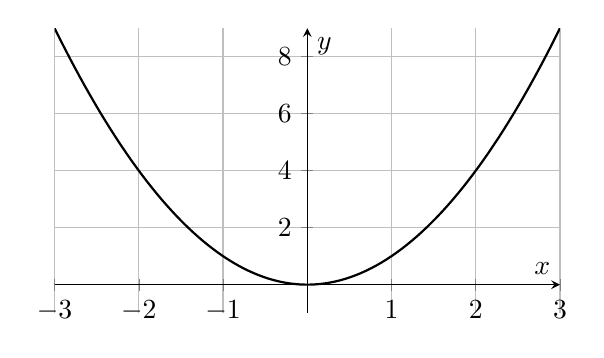
\begin{tikzpicture}
\begin{axis}[
    width=8cm,
    height=5.2cm,
    axis lines=middle,
    xmin=-3,xmax=3,
    ymin=-1,ymax=9,
    xlabel={$x$},
    ylabel={$y$},
    samples=100,
    grid=major
]
\addplot[domain=-3:3,thick] {x^2};
\end{axis}
\end{tikzpicture}
\end{center}

%%%%%%%%%%%%%%%%%%%%%%%%%%%%%%%%%%%%%%%%%%%%%%%%%%%%%%%%%%%%
\subsection{Vertical Line Test}
\label{subsec:vertical-line-test}
%%%%%%%%%%%%%%%%%%%%%%%%%%%%%%%%%%%%%%%%%%%%%%%%%%%%%%%%%%%%

A graph represents \(y\) as a function of \(x\) exactly when each permitted
\(x\)-value corresponds to at most one \(y\)-value.

\begin{principle}[Vertical Line Test]
A plane curve represents \(y\) as a function of \(x\) if and only if every
vertical line intersects the graph at most once.
\end{principle}

A circle such as

\[ x^2+y^2=1 \]

fails the vertical line test because many vertical lines intersect the
circle twice.

%%%%%%%%%%%%%%%%%%%%%%%%%%%%%%%%%%%%%%%%%%%%%%%%%%%%%%%%%%%%
\subsection{Domain}
\label{subsec:analysis-domain}
%%%%%%%%%%%%%%%%%%%%%%%%%%%%%%%%%%%%%%%%%%%%%%%%%%%%%%%%%%%%

For a function given algebraically, the domain consists of inputs for which
the expression is defined.

Common restrictions arise from:

\begin{itemize}
    \item division by zero;
    \item even roots of negative real numbers;
    \item logarithms of nonpositive numbers;
    \item restrictions imposed by an application.
\end{itemize}

%%%%%%%%%%%%%%%%%%%%%%%%%%%%%%%%%%%%%%%%%%%%%%%%%%%%%%%%%%%%
\subsection{Rational Domain Restrictions}
\label{subsec:rational-domain-restrictions}
%%%%%%%%%%%%%%%%%%%%%%%%%%%%%%%%%%%%%%%%%%%%%%%%%%%%%%%%%%%%

For

\[ f(x)=\frac{1}{x-3}, \]

the denominator cannot equal zero.

Thus

\[ x-3\neq0, \]

so

\[ x\neq3. \]

Therefore,

\[ \dom(f)=(-\infty,3)\cup(3,\infty). \]

%%%%%%%%%%%%%%%%%%%%%%%%%%%%%%%%%%%%%%%%%%%%%%%%%%%%%%%%%%%%
\subsection{Radical Domain Restrictions}
\label{subsec:radical-domain-restrictions}
%%%%%%%%%%%%%%%%%%%%%%%%%%%%%%%%%%%%%%%%%%%%%%%%%%%%%%%%%%%%

For

\[ f(x)=\sqrt{x-4}, \]

the radicand must satisfy

\[ x-4\geq0. \]

Hence

\[ x\geq4. \]

Therefore,

\[ \dom(f)=[4,\infty). \]

%%%%%%%%%%%%%%%%%%%%%%%%%%%%%%%%%%%%%%%%%%%%%%%%%%%%%%%%%%%%
\subsection{Logarithmic Domain Restrictions}
\label{subsec:log-domain-restrictions}
%%%%%%%%%%%%%%%%%%%%%%%%%%%%%%%%%%%%%%%%%%%%%%%%%%%%%%%%%%%%

For

\[ f(x)=\ln(x+2), \]

the logarithm requires

\[ x+2>0. \]

Thus

\[ x>-2, \]

and

\[ \dom(f)=(-2,\infty). \]

The notation

\[ \ln x \]

is read ``natural logarithm of \(x\).''

The logarithm will be developed in detail later in this section.

%%%%%%%%%%%%%%%%%%%%%%%%%%%%%%%%%%%%%%%%%%%%%%%%%%%%%%%%%%%%
\subsection{Worked Example: Finding a Domain}
\label{subsec:worked-domain}
%%%%%%%%%%%%%%%%%%%%%%%%%%%%%%%%%%%%%%%%%%%%%%%%%%%%%%%%%%%%

\begin{workedexamplebox}{Domain of a Composite Algebraic Expression}

Find the real domain of

\[ f(x)=\frac{\sqrt{x+1}}{x-2}. \]

\begin{tabularx}{\textwidth}{@{}>{\raggedright\arraybackslash}p{0.42\textwidth}X@{}}
Require the square root to be real. &
\(x+1\geq0\Rightarrow x\geq-1\)\\
Require the denominator to be nonzero. &
\(x-2\neq0\Rightarrow x\neq2\)\\
Combine the restrictions. &
\(x\geq-1\) with \(x\neq2\)
\end{tabularx}

\begin{answerbox}
\[ \boxed{\dom(f)=[-1,2)\cup(2,\infty).} \]
\end{answerbox}
\end{workedexamplebox}

%%%%%%%%%%%%%%%%%%%%%%%%%%%%%%%%%%%%%%%%%%%%%%%%%%%%%%%%%%%%
\subsection{Range}
\label{subsec:analysis-range}
%%%%%%%%%%%%%%%%%%%%%%%%%%%%%%%%%%%%%%%%%%%%%%%%%%%%%%%%%%%%

The range of a real-valued function is the set

\[ \{f(x):x\in\dom(f)\}. \]

For example,

\[ f(x)=x^2 \]

has domain

\[ \R \]

and range

\[ [0,\infty). \]

The domain asks:

\begin{quote}
Which inputs are allowed?
\end{quote}

The range asks:

\begin{quote}
Which outputs are possible?
\end{quote}

%%%%%%%%%%%%%%%%%%%%%%%%%%%%%%%%%%%%%%%%%%%%%%%%%%%%%%%%%%%%
\subsection{Intercepts}
\label{subsec:function-intercepts}
%%%%%%%%%%%%%%%%%%%%%%%%%%%%%%%%%%%%%%%%%%%%%%%%%%%%%%%%%%%%

An \(x\)-intercept occurs where

\[ f(x)=0. \]

Such inputs are called \emph{zeros} or \emph{roots} of the function.

A \(y\)-intercept occurs at

\[ x=0, \]

provided \(0\) belongs to the domain.

Thus the \(y\)-intercept is

\[ (0,f(0)). \]

For

\[ f(x)=x^2-4, \]

the zeros satisfy

\[ x^2-4=0, \]

so

\[ x=\pm2. \]

The \(x\)-intercepts are

\[ (-2,0),\qquad(2,0). \]

The \(y\)-intercept is

\[ (0,-4). \]

%%%%%%%%%%%%%%%%%%%%%%%%%%%%%%%%%%%%%%%%%%%%%%%%%%%%%%%%%%%%
\subsection{Increasing and Decreasing Functions}
\label{subsec:increasing-decreasing}
%%%%%%%%%%%%%%%%%%%%%%%%%%%%%%%%%%%%%%%%%%%%%%%%%%%%%%%%%%%%

\begin{definitionbox}{Increasing Function}
A function \(f\) is \emph{increasing} on an interval \(I\) if
\[ x_1<x_2\Longrightarrow f(x_1)\leq f(x_2) \]
for \(x_1,x_2\in I\).
\end{definitionbox}

\begin{definitionbox}{Decreasing Function}
A function \(f\) is \emph{decreasing} on an interval \(I\) if
\[ x_1<x_2\Longrightarrow f(x_1)\geq f(x_2). \]
\end{definitionbox}

Some texts distinguish strictly increasing and strictly decreasing by using
strict inequalities.

These ideas become fundamental when derivatives are introduced.

%%%%%%%%%%%%%%%%%%%%%%%%%%%%%%%%%%%%%%%%%%%%%%%%%%%%%%%%%%%%
\subsection{Local and Global Extrema}
\label{subsec:precalculus-extrema}
%%%%%%%%%%%%%%%%%%%%%%%%%%%%%%%%%%%%%%%%%%%%%%%%%%%%%%%%%%%%

A function may attain large or small values relative to nearby points or
relative to its entire domain.

A \emph{local maximum} is a value larger than nearby function values.

A \emph{local minimum} is smaller than nearby function values.

An \emph{absolute maximum} is the largest value attained on the entire
domain under consideration.

An \emph{absolute minimum} is the smallest.

These concepts will later be analyzed using derivatives.

%%%%%%%%%%%%%%%%%%%%%%%%%%%%%%%%%%%%%%%%%%%%%%%%%%%%%%%%%%%%
\subsection{Bounded Functions}
\label{subsec:bounded-functions}
%%%%%%%%%%%%%%%%%%%%%%%%%%%%%%%%%%%%%%%%%%%%%%%%%%%%%%%%%%%%

\begin{definitionbox}{Bounded Above}
A real-valued function \(f\) is \emph{bounded above} if there exists
\(M\in\R\) such that
\[ f(x)\leq M \]
for every \(x\) in its domain.
\end{definitionbox}

Similarly, \(f\) is bounded below if there exists \(m\in\R\) such that

\[ m\leq f(x). \]

It is \emph{bounded} if it is both bounded above and bounded below.

For example,

\[ \sin x \]

is bounded because

\[ -1\leq\sin x\leq1. \]

%%%%%%%%%%%%%%%%%%%%%%%%%%%%%%%%%%%%%%%%%%%%%%%%%%%%%%%%%%%%
\subsection{Even Functions}
\label{subsec:even-functions}
%%%%%%%%%%%%%%%%%%%%%%%%%%%%%%%%%%%%%%%%%%%%%%%%%%%%%%%%%%%%

\begin{definitionbox}{Even Function}
A function \(f\) is \emph{even} if
\[ f(-x)=f(x) \]
whenever both sides are defined.
\end{definitionbox}

The graph of an even function is symmetric about the \(y\)-axis.

For example,

\[ f(x)=x^2 \]

is even because

\[ f(-x)=(-x)^2=x^2=f(x). \]

%%%%%%%%%%%%%%%%%%%%%%%%%%%%%%%%%%%%%%%%%%%%%%%%%%%%%%%%%%%%
\subsection{Odd Functions}
\label{subsec:odd-functions}
%%%%%%%%%%%%%%%%%%%%%%%%%%%%%%%%%%%%%%%%%%%%%%%%%%%%%%%%%%%%

\begin{definitionbox}{Odd Function}
A function \(f\) is \emph{odd} if
\[ f(-x)=-f(x). \]
\end{definitionbox}

The graph of an odd function has rotational symmetry of \(180^\circ\) about
the origin.

For example,

\[ f(x)=x^3 \]

is odd because

\[ f(-x)=(-x)^3=-x^3=-f(x). \]

%%%%%%%%%%%%%%%%%%%%%%%%%%%%%%%%%%%%%%%%%%%%%%%%%%%%%%%%%%%%
\subsection{Parent Functions}
\label{subsec:parent-functions}
%%%%%%%%%%%%%%%%%%%%%%%%%%%%%%%%%%%%%%%%%%%%%%%%%%%%%%%%%%%%

Many functions are transformations of a small collection of fundamental
graphs.

Common parent functions include

\[
f(x)=x,\qquad
f(x)=x^2,\qquad
f(x)=x^3,
\]

\[
f(x)=\sqrt{x},\qquad
f(x)=|x|,\qquad
f(x)=\frac1x,
\]

\[
f(x)=a^x,\qquad
f(x)=\log_a x,
\]

and the trigonometric functions.

Understanding their shapes makes more complicated graphs easier to analyze.

%%%%%%%%%%%%%%%%%%%%%%%%%%%%%%%%%%%%%%%%%%%%%%%%%%%%%%%%%%%%
\subsection{Function Transformations}
\label{subsec:function-transformations}
%%%%%%%%%%%%%%%%%%%%%%%%%%%%%%%%%%%%%%%%%%%%%%%%%%%%%%%%%%%%

Suppose a function \(f\) is transformed into

\[ g(x)=Af(B(x-C))+D. \]

The constants affect the graph in predictable ways.

\begin{center}
\begin{tabularx}{0.9\textwidth}{@{}lX@{}}
\toprule
\textbf{Parameter} & \textbf{Typical Effect}\\
\midrule
\(A\) & vertical scaling and possible reflection across the \(x\)-axis\\
\(B\) & horizontal scaling and possible reflection across the \(y\)-axis\\
\(C\) & horizontal translation\\
\(D\) & vertical translation\\
\bottomrule
\end{tabularx}
\end{center}

%%%%%%%%%%%%%%%%%%%%%%%%%%%%%%%%%%%%%%%%%%%%%%%%%%%%%%%%%%%%
\subsection{Vertical Translations}
\label{subsec:vertical-translations}
%%%%%%%%%%%%%%%%%%%%%%%%%%%%%%%%%%%%%%%%%%%%%%%%%%%%%%%%%%%%

The transformation

\[ g(x)=f(x)+D \]

moves the graph vertically.

If \(D>0\), the graph shifts upward.

If \(D<0\), it shifts downward.

For example,

\[ g(x)=x^2+3 \]

is the parabola \(y=x^2\) shifted upward \(3\) units.

%%%%%%%%%%%%%%%%%%%%%%%%%%%%%%%%%%%%%%%%%%%%%%%%%%%%%%%%%%%%
\subsection{Horizontal Translations}
\label{subsec:horizontal-translations}
%%%%%%%%%%%%%%%%%%%%%%%%%%%%%%%%%%%%%%%%%%%%%%%%%%%%%%%%%%%%

The transformation

\[ g(x)=f(x-C) \]

moves the graph horizontally.

If \(C>0\), the graph shifts right by \(C\).

If \(C<0\), it shifts left by \(|C|\).

Thus

\[ g(x)=(x-4)^2 \]

is \(y=x^2\) shifted right \(4\) units.

The sign appears reversed inside the function because inputs must reach the
same original value after the shift.

%%%%%%%%%%%%%%%%%%%%%%%%%%%%%%%%%%%%%%%%%%%%%%%%%%%%%%%%%%%%
\subsection{Reflections}
\label{subsec:function-reflections}
%%%%%%%%%%%%%%%%%%%%%%%%%%%%%%%%%%%%%%%%%%%%%%%%%%%%%%%%%%%%

The transformation

\[ g(x)=-f(x) \]

reflects the graph across the \(x\)-axis.

The transformation

\[ g(x)=f(-x) \]

reflects the graph across the \(y\)-axis.

For example,

\[ y=-x^2 \]

is the reflection of

\[ y=x^2 \]

across the \(x\)-axis.

%%%%%%%%%%%%%%%%%%%%%%%%%%%%%%%%%%%%%%%%%%%%%%%%%%%%%%%%%%%%
\subsection{Vertical Scaling}
\label{subsec:vertical-scaling}
%%%%%%%%%%%%%%%%%%%%%%%%%%%%%%%%%%%%%%%%%%%%%%%%%%%%%%%%%%%%

For

\[ g(x)=Af(x), \]

all \(y\)-values are multiplied by \(A\).

If

\[ |A|>1, \]

the graph is vertically stretched.

If

\[ 0<|A|<1, \]

the graph is vertically compressed.

If \(A<0\), a reflection across the \(x\)-axis also occurs.

%%%%%%%%%%%%%%%%%%%%%%%%%%%%%%%%%%%%%%%%%%%%%%%%%%%%%%%%%%%%
\subsection{Horizontal Scaling}
\label{subsec:horizontal-scaling}
%%%%%%%%%%%%%%%%%%%%%%%%%%%%%%%%%%%%%%%%%%%%%%%%%%%%%%%%%%%%

For

\[ g(x)=f(Bx), \]

horizontal distances are scaled by

\[ \frac{1}{|B|}. \]

Thus if

\[ |B|>1, \]

the graph is horizontally compressed.

If

\[ 0<|B|<1, \]

the graph is horizontally stretched.

This reciprocal behavior is a frequent source of mistakes.

%%%%%%%%%%%%%%%%%%%%%%%%%%%%%%%%%%%%%%%%%%%%%%%%%%%%%%%%%%%%
\subsection{Worked Example: Graph Transformations}
\label{subsec:worked-transformations}
%%%%%%%%%%%%%%%%%%%%%%%%%%%%%%%%%%%%%%%%%%%%%%%%%%%%%%%%%%%%

\begin{workedexamplebox}{Transforming a Parabola}

Describe the transformations from

\[ f(x)=x^2 \]

to

\[ g(x)=-2(x-3)^2+4. \]

\begin{tabularx}{\textwidth}{@{}>{\raggedright\arraybackslash}p{0.42\textwidth}X@{}}
The expression \(x-3\) shifts horizontally. &
Shift right \(3\).\\
The factor \(2\) outside scales vertically. &
Vertical stretch by factor \(2\).\\
The negative sign outside reflects vertically. &
Reflect across the \(x\)-axis.\\
The \(+4\) shifts vertically. &
Shift upward \(4\).
\end{tabularx}

\begin{answerbox}
\[
\boxed{\text{Right }3,\quad
\text{vertical stretch by }2,\quad
\text{reflect across \(x\)-axis},\quad
\text{up }4.}
\]
\end{answerbox}
\end{workedexamplebox}

%%%%%%%%%%%%%%%%%%%%%%%%%%%%%%%%%%%%%%%%%%%%%%%%%%%%%%%%%%%%
\subsection{Arithmetic Operations on Functions}
\label{subsec:function-arithmetic}
%%%%%%%%%%%%%%%%%%%%%%%%%%%%%%%%%%%%%%%%%%%%%%%%%%%%%%%%%%%%

Given functions \(f\) and \(g\), define

\[ (f+g)(x)=f(x)+g(x), \]

\[ (f-g)(x)=f(x)-g(x), \]

\[ (fg)(x)=f(x)g(x), \]

and, when \(g(x)\neq0\),

\[ \left(\frac fg\right)(x)=\frac{f(x)}{g(x)}. \]

The domain of the resulting function consists of inputs where all required
expressions are defined.

%%%%%%%%%%%%%%%%%%%%%%%%%%%%%%%%%%%%%%%%%%%%%%%%%%%%%%%%%%%%
\subsection{Composition of Functions}
\label{subsec:analysis-composition}
%%%%%%%%%%%%%%%%%%%%%%%%%%%%%%%%%%%%%%%%%%%%%%%%%%%%%%%%%%%%

\begin{definitionbox}{Composition}
If \(g(x)\) produces inputs allowed by \(f\), the composition
\[ (f\circ g)(x)=f(g(x)) \]
is obtained by applying \(g\) first and \(f\) second.
\end{definitionbox}

The symbol

\[ \circ \]

is read ``composed with.''

Thus

\[ f\circ g \]

is read ``\(f\) composed with \(g\).''

%%%%%%%%%%%%%%%%%%%%%%%%%%%%%%%%%%%%%%%%%%%%%%%%%%%%%%%%%%%%
\subsection{Worked Example: Composition}
\label{subsec:worked-function-composition}
%%%%%%%%%%%%%%%%%%%%%%%%%%%%%%%%%%%%%%%%%%%%%%%%%%%%%%%%%%%%

\begin{workedexamplebox}{Composing Two Functions}

Let

\[ f(x)=x^2+1,\qquad g(x)=3x-2. \]

Find \(f\circ g\) and \(g\circ f\).

\begin{tabularx}{\textwidth}{@{}>{\raggedright\arraybackslash}p{0.42\textwidth}X@{}}
Substitute \(g(x)\) into \(f\). &
\((f\circ g)(x)=(3x-2)^2+1\)\\
Expand. &
\((f\circ g)(x)=9x^2-12x+5\)\\[2mm]
Substitute \(f(x)\) into \(g\). &
\((g\circ f)(x)=3(x^2+1)-2\)\\
Simplify. &
\((g\circ f)(x)=3x^2+1\)
\end{tabularx}

\begin{answerbox}
\[ \boxed{(f\circ g)(x)=9x^2-12x+5,\qquad
(g\circ f)(x)=3x^2+1.} \]
\end{answerbox}
\end{workedexamplebox}

%%%%%%%%%%%%%%%%%%%%%%%%%%%%%%%%%%%%%%%%%%%%%%%%%%%%%%%%%%%%
\subsection{Composition Is Not Commutative}
\label{subsec:composition-not-commutative}
%%%%%%%%%%%%%%%%%%%%%%%%%%%%%%%%%%%%%%%%%%%%%%%%%%%%%%%%%%%%

In general,

\[ f\circ g\neq g\circ f. \]

The order of composition matters.

This resembles matrix multiplication and many other noncommutative
operations.

%%%%%%%%%%%%%%%%%%%%%%%%%%%%%%%%%%%%%%%%%%%%%%%%%%%%%%%%%%%%
\subsection{One-to-One Functions}
\label{subsec:one-to-one-analysis}
%%%%%%%%%%%%%%%%%%%%%%%%%%%%%%%%%%%%%%%%%%%%%%%%%%%%%%%%%%%%

\begin{definitionbox}{One-to-One Function}
A function \(f\) is \emph{one-to-one}, or injective, if
\[ f(x_1)=f(x_2)\Longrightarrow x_1=x_2. \]
\end{definitionbox}

Equivalently, distinct inputs produce distinct outputs.

Graphically, one-to-one behavior is tested with horizontal lines.

%%%%%%%%%%%%%%%%%%%%%%%%%%%%%%%%%%%%%%%%%%%%%%%%%%%%%%%%%%%%
\subsection{Horizontal Line Test}
\label{subsec:horizontal-line-test}
%%%%%%%%%%%%%%%%%%%%%%%%%%%%%%%%%%%%%%%%%%%%%%%%%%%%%%%%%%%%

\begin{principle}[Horizontal Line Test]
A function is one-to-one if and only if every horizontal line intersects
its graph at most once.
\end{principle}

For example,

\[ f(x)=x^3 \]

is one-to-one on \(\R\).

However,

\[ f(x)=x^2 \]

is not one-to-one on \(\R\), since

\[ f(-1)=f(1)=1. \]

%%%%%%%%%%%%%%%%%%%%%%%%%%%%%%%%%%%%%%%%%%%%%%%%%%%%%%%%%%%%
\subsection{Inverse Functions}
\label{subsec:inverse-functions-analysis}
%%%%%%%%%%%%%%%%%%%%%%%%%%%%%%%%%%%%%%%%%%%%%%%%%%%%%%%%%%%%

A one-to-one function can be reversed.

\begin{definitionbox}{Inverse Function}
If \(f:A\to B\) is bijective, its inverse is the function
\[ f^{-1}:B\to A \]
satisfying
\[ f^{-1}(f(x))=x \]
and
\[ f(f^{-1}(y))=y. \]
\end{definitionbox}

The notation

\[ f^{-1} \]

is read ``\(f\) inverse.''

It does \emph{not} mean

\[ \frac1{f}. \]

%%%%%%%%%%%%%%%%%%%%%%%%%%%%%%%%%%%%%%%%%%%%%%%%%%%%%%%%%%%%
\subsection{Finding an Inverse Algebraically}
\label{subsec:finding-inverses}
%%%%%%%%%%%%%%%%%%%%%%%%%%%%%%%%%%%%%%%%%%%%%%%%%%%%%%%%%%%%

To find an inverse:

\begin{enumerate}
    \item write \(y=f(x)\);
    \item solve for \(x\) in terms of \(y\);
    \item exchange \(x\) and \(y\);
    \item write the result as \(f^{-1}(x)\).
\end{enumerate}

%%%%%%%%%%%%%%%%%%%%%%%%%%%%%%%%%%%%%%%%%%%%%%%%%%%%%%%%%%%%
\subsection{Worked Example: Finding an Inverse}
\label{subsec:worked-inverse}
%%%%%%%%%%%%%%%%%%%%%%%%%%%%%%%%%%%%%%%%%%%%%%%%%%%%%%%%%%%%

\begin{workedexamplebox}{Finding an Inverse Function}

Let

\[ f(x)=3x-5. \]

Find \(f^{-1}(x)\).

\begin{tabularx}{\textwidth}{@{}>{\raggedright\arraybackslash}p{0.42\textwidth}X@{}}
Write the function using \(y\). &
\(y=3x-5\)\\
Solve for \(x\). &
\(y+5=3x\)\\
Divide by \(3\). &
\(x=\dfrac{y+5}{3}\)\\
Exchange variables. &
\(y=\dfrac{x+5}{3}\)
\end{tabularx}

\begin{answerbox}
\[ \boxed{f^{-1}(x)=\frac{x+5}{3}.} \]
\end{answerbox}
\end{workedexamplebox}

%%%%%%%%%%%%%%%%%%%%%%%%%%%%%%%%%%%%%%%%%%%%%%%%%%%%%%%%%%%%
\subsection{Graphs of Inverse Functions}
\label{subsec:inverse-function-graphs}
%%%%%%%%%%%%%%%%%%%%%%%%%%%%%%%%%%%%%%%%%%%%%%%%%%%%%%%%%%%%

The graph of \(f^{-1}\) is the reflection of the graph of \(f\) across the
line

\[ y=x. \]

This occurs because the ordered pair

\[ (a,b) \]

on the graph of \(f\) becomes

\[ (b,a) \]

on the graph of \(f^{-1}\).

%%%%%%%%%%%%%%%%%%%%%%%%%%%%%%%%%%%%%%%%%%%%%%%%%%%%%%%%%%%%
\subsection{Polynomial Functions}
\label{subsec:polynomial-functions-analysis}
%%%%%%%%%%%%%%%%%%%%%%%%%%%%%%%%%%%%%%%%%%%%%%%%%%%%%%%%%%%%

\begin{definitionbox}{Polynomial Function}
A \emph{polynomial function} has the form
\[ P(x)=a_nx^n+a_{n-1}x^{n-1}+\cdots+a_1x+a_0, \]
where \(n\) is a nonnegative integer and \(a_n\neq0\).
\end{definitionbox}

The integer \(n\) is the degree.

Polynomial functions are defined for every real number:

\[ \dom(P)=\R. \]

%%%%%%%%%%%%%%%%%%%%%%%%%%%%%%%%%%%%%%%%%%%%%%%%%%%%%%%%%%%%
\subsection{Common Polynomial Degrees}
\label{subsec:common-polynomials}
%%%%%%%%%%%%%%%%%%%%%%%%%%%%%%%%%%%%%%%%%%%%%%%%%%%%%%%%%%%%

\begin{center}
\begin{tabularx}{0.8\textwidth}{@{}clX@{}}
\toprule
\textbf{Degree} & \textbf{Name} & \textbf{Typical Form}\\
\midrule
\(0\) & constant & \(a\)\\
\(1\) & linear & \(ax+b\)\\
\(2\) & quadratic & \(ax^2+bx+c\)\\
\(3\) & cubic & \(ax^3+bx^2+cx+d\)\\
\(4\) & quartic & \(ax^4+\cdots\)\\
\(5\) & quintic & \(ax^5+\cdots\)\\
\bottomrule
\end{tabularx}
\end{center}

%%%%%%%%%%%%%%%%%%%%%%%%%%%%%%%%%%%%%%%%%%%%%%%%%%%%%%%%%%%%
\subsection{Linear Functions}
\label{subsec:linear-functions-analysis}
%%%%%%%%%%%%%%%%%%%%%%%%%%%%%%%%%%%%%%%%%%%%%%%%%%%%%%%%%%%%

A linear function has the form

\[ f(x)=mx+b. \]

The constant \(m\) is the slope and \(b\) is the \(y\)-intercept.

Slope is

\[ m=\frac{\Delta y}{\Delta x}. \]

The uppercase Greek letter

\[ \Delta \]

is delta, pronounced ``DEL-tuh.''

In this context,

\[ \Delta y \]

means ``change in \(y\),'' and

\[ \Delta x \]

means ``change in \(x\).''

%%%%%%%%%%%%%%%%%%%%%%%%%%%%%%%%%%%%%%%%%%%%%%%%%%%%%%%%%%%%
\subsection{Quadratic Functions}
\label{subsec:quadratic-functions-analysis}
%%%%%%%%%%%%%%%%%%%%%%%%%%%%%%%%%%%%%%%%%%%%%%%%%%%%%%%%%%%%

A quadratic function has the form

\[ f(x)=ax^2+bx+c,\qquad a\neq0. \]

Its graph is a parabola.

Vertex form is

\[ f(x)=a(x-h)^2+k. \]

The vertex is

\[ (h,k). \]

The axis of symmetry is

\[ x=h. \]

If \(a>0\), the parabola opens upward.

If \(a<0\), it opens downward.

%%%%%%%%%%%%%%%%%%%%%%%%%%%%%%%%%%%%%%%%%%%%%%%%%%%%%%%%%%%%
\subsection{Zeros and Factors}
\label{subsec:polynomial-zeros-factors}
%%%%%%%%%%%%%%%%%%%%%%%%%%%%%%%%%%%%%%%%%%%%%%%%%%%%%%%%%%%%

For a polynomial \(P(x)\),

\[ P(r)=0 \]

if and only if

\[ x-r \]

is a factor of \(P(x)\).

This is the \emph{Factor Theorem}.

Zeros of the polynomial correspond to \(x\)-intercepts of its graph.

%%%%%%%%%%%%%%%%%%%%%%%%%%%%%%%%%%%%%%%%%%%%%%%%%%%%%%%%%%%%
\subsection{Multiplicity}
\label{subsec:zero-multiplicity}
%%%%%%%%%%%%%%%%%%%%%%%%%%%%%%%%%%%%%%%%%%%%%%%%%%%%%%%%%%%%

If

\[ P(x)=(x-r)^mQ(x), \qquad Q(r)\neq0, \]

then \(r\) is a zero of multiplicity \(m\).

If \(m\) is odd, the graph typically crosses the \(x\)-axis at \(r\).

If \(m\) is even, the graph typically touches the axis and turns around.

%%%%%%%%%%%%%%%%%%%%%%%%%%%%%%%%%%%%%%%%%%%%%%%%%%%%%%%%%%%%
\subsection{Polynomial End Behavior}
\label{subsec:polynomial-end-behavior}
%%%%%%%%%%%%%%%%%%%%%%%%%%%%%%%%%%%%%%%%%%%%%%%%%%%%%%%%%%%%

For large \(|x|\), the leading term

\[ a_nx^n \]

dominates a polynomial's behavior.

Thus end behavior depends primarily on:

\begin{itemize}
    \item whether the degree is even or odd;
    \item whether the leading coefficient is positive or negative.
\end{itemize}

\begin{center}
\begin{tabularx}{0.92\textwidth}{@{}lll@{}}
\toprule
\textbf{Degree} & \textbf{Leading Coefficient} & \textbf{End Behavior}\\
\midrule
even & positive & both ends rise\\
even & negative & both ends fall\\
odd & positive & left falls, right rises\\
odd & negative & left rises, right falls\\
\bottomrule
\end{tabularx}
\end{center}

%%%%%%%%%%%%%%%%%%%%%%%%%%%%%%%%%%%%%%%%%%%%%%%%%%%%%%%%%%%%
\subsection{Rational Functions}
\label{subsec:rational-functions-analysis}
%%%%%%%%%%%%%%%%%%%%%%%%%%%%%%%%%%%%%%%%%%%%%%%%%%%%%%%%%%%%

\begin{definitionbox}{Rational Function}
A \emph{rational function} has the form
\[ R(x)=\frac{P(x)}{Q(x)}, \]
where \(P\) and \(Q\) are polynomials and \(Q(x)\neq0\).
\end{definitionbox}

The domain excludes zeros of \(Q\).

Rational functions introduce important phenomena such as:

\begin{itemize}
    \item holes;
    \item vertical asymptotes;
    \item horizontal asymptotes;
    \item oblique asymptotes.
\end{itemize}

%%%%%%%%%%%%%%%%%%%%%%%%%%%%%%%%%%%%%%%%%%%%%%%%%%%%%%%%%%%%
\subsection{Vertical Asymptotes}
\label{subsec:vertical-asymptotes}
%%%%%%%%%%%%%%%%%%%%%%%%%%%%%%%%%%%%%%%%%%%%%%%%%%%%%%%%%%%%

A vertical line

\[ x=a \]

is a vertical asymptote when the magnitude of \(f(x)\) grows without bound
as \(x\) approaches \(a\) from at least one side.

For the reciprocal function

\[ f(x)=\frac1x, \]

the line

\[ x=0 \]

is a vertical asymptote.

\begin{center}
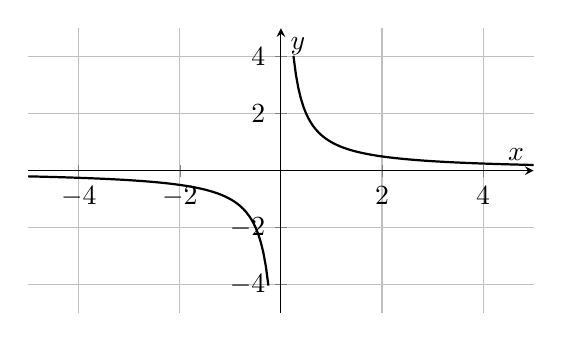
\begin{tikzpicture}
\begin{axis}[
    width=8cm,
    height=5.2cm,
    axis lines=middle,
    xmin=-5,xmax=5,
    ymin=-5,ymax=5,
    xlabel={$x$},
    ylabel={$y$},
    samples=100,
    restrict y to domain=-5:5,
    grid=major
]
\addplot[domain=-5:-0.15,thick] {1/x};
\addplot[domain=0.15:5,thick] {1/x};
\end{axis}
\end{tikzpicture}
\end{center}

%%%%%%%%%%%%%%%%%%%%%%%%%%%%%%%%%%%%%%%%%%%%%%%%%%%%%%%%%%%%
\subsection{Horizontal Asymptotes}
\label{subsec:horizontal-asymptotes}
%%%%%%%%%%%%%%%%%%%%%%%%%%%%%%%%%%%%%%%%%%%%%%%%%%%%%%%%%%%%

A horizontal line

\[ y=L \]

describes the value approached by a function as

\[ x\to\infty \]

or

\[ x\to-\infty. \]

The notation

\[ x\to\infty \]

is read ``\(x\) approaches infinity.''

For

\[ f(x)=\frac1x, \]

the graph approaches

\[ y=0 \]

as \(|x|\) becomes large.

Formal limit notation will be developed in Single-Variable Calculus.

%%%%%%%%%%%%%%%%%%%%%%%%%%%%%%%%%%%%%%%%%%%%%%%%%%%%%%%%%%%%
\subsection{Holes and Removable Factors}
\label{subsec:rational-holes}
%%%%%%%%%%%%%%%%%%%%%%%%%%%%%%%%%%%%%%%%%%%%%%%%%%%%%%%%%%%%

Consider

\[ f(x)=\frac{x^2-1}{x-1}. \]

Factor the numerator:

\[ f(x)=\frac{(x-1)(x+1)}{x-1}. \]

For \(x\neq1\),

\[ f(x)=x+1. \]

However, the original function is undefined at

\[ x=1. \]

Thus the graph is the line

\[ y=x+1 \]

with a hole at

\[ (1,2). \]

This type of behavior will later motivate removable discontinuities.

%%%%%%%%%%%%%%%%%%%%%%%%%%%%%%%%%%%%%%%%%%%%%%%%%%%%%%%%%%%%
\subsection{Radical Functions}
\label{subsec:radical-functions-analysis}
%%%%%%%%%%%%%%%%%%%%%%%%%%%%%%%%%%%%%%%%%%%%%%%%%%%%%%%%%%%%

A radical function contains roots of expressions involving the variable.

Examples include

\[ f(x)=\sqrt{x}, \]

\[ g(x)=\sqrt{x+3}, \]

and

\[ h(x)=\sqrt[3]{x}. \]

Even roots impose nonnegative-radicand restrictions over the real numbers.

Odd roots are defined for every real input.

%%%%%%%%%%%%%%%%%%%%%%%%%%%%%%%%%%%%%%%%%%%%%%%%%%%%%%%%%%%%
\subsection{Absolute-Value Functions}
\label{subsec:absolute-value-functions}
%%%%%%%%%%%%%%%%%%%%%%%%%%%%%%%%%%%%%%%%%%%%%%%%%%%%%%%%%%%%

The absolute value function is

\[
|x|=
\begin{cases}
x, & x\geq0,\\
-x, & x<0.
\end{cases}
\]

Its graph has a V-shape.

\begin{center}
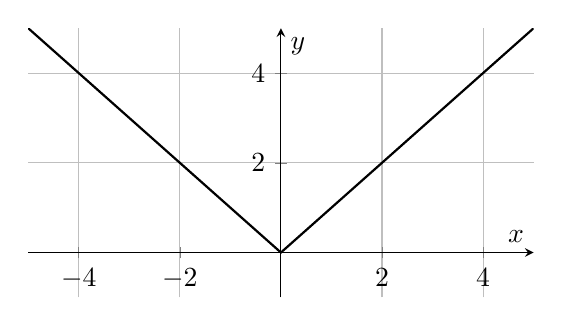
\begin{tikzpicture}
\begin{axis}[
    width=8cm,
    height=5cm,
    axis lines=middle,
    xmin=-5,xmax=5,
    ymin=-1,ymax=5,
    xlabel={$x$},
    ylabel={$y$},
    grid=major
]
\addplot[domain=-5:5,thick] {abs(x)};
\end{axis}
\end{tikzpicture}
\end{center}

Geometrically,

\[ |x| \]

represents the distance from \(x\) to \(0\) on the real number line.

More generally,

\[ |x-a| \]

represents the distance between \(x\) and \(a\).

%%%%%%%%%%%%%%%%%%%%%%%%%%%%%%%%%%%%%%%%%%%%%%%%%%%%%%%%%%%%
\subsection{Piecewise-Defined Functions}
\label{subsec:piecewise-functions}
%%%%%%%%%%%%%%%%%%%%%%%%%%%%%%%%%%%%%%%%%%%%%%%%%%%%%%%%%%%%

A function may use different rules on different portions of its domain.

For example,

\[
f(x)=
\begin{cases}
x^2, & x<0,\\
2x+1, & x\geq0.
\end{cases}
\]

This is called a \emph{piecewise-defined function}.

Piecewise functions are essential in modeling situations where behavior
changes at thresholds.

They also become central when studying continuity and differentiability.

%%%%%%%%%%%%%%%%%%%%%%%%%%%%%%%%%%%%%%%%%%%%%%%%%%%%%%%%%%%%
\subsection{Greatest Integer and Floor Functions}
\label{subsec:floor-function}
%%%%%%%%%%%%%%%%%%%%%%%%%%%%%%%%%%%%%%%%%%%%%%%%%%%%%%%%%%%%

The floor function is

\[ f(x)=\floor{x}. \]

It assigns the greatest integer less than or equal to \(x\).

For example,

\[ \floor{3.7}=3, \]

and

\[ \floor{-1.2}=-2. \]

The graph is a step function.

Such functions provide important examples of discontinuous behavior.

%%%%%%%%%%%%%%%%%%%%%%%%%%%%%%%%%%%%%%%%%%%%%%%%%%%%%%%%%%%%
\subsection{Exponential Functions}
\label{subsec:exponential-functions-analysis}
%%%%%%%%%%%%%%%%%%%%%%%%%%%%%%%%%%%%%%%%%%%%%%%%%%%%%%%%%%%%

\begin{definitionbox}{Exponential Function}
An \emph{exponential function} has the form
\[ f(x)=a^x, \]
where
\[ a>0,\qquad a\neq1. \]
\end{definitionbox}

The variable appears in the exponent.

This distinguishes exponential functions from power functions such as

\[ x^2. \]

%%%%%%%%%%%%%%%%%%%%%%%%%%%%%%%%%%%%%%%%%%%%%%%%%%%%%%%%%%%%
\subsection{Exponential Growth and Decay}
\label{subsec:exponential-growth-decay}
%%%%%%%%%%%%%%%%%%%%%%%%%%%%%%%%%%%%%%%%%%%%%%%%%%%%%%%%%%%%

If

\[ a>1, \]

then

\[ f(x)=a^x \]

represents exponential growth.

If

\[ 0<a<1, \]

then it represents exponential decay.

For every valid base \(a\),

\[ a^0=1. \]

Thus all basic exponential graphs pass through

\[ (0,1). \]

%%%%%%%%%%%%%%%%%%%%%%%%%%%%%%%%%%%%%%%%%%%%%%%%%%%%%%%%%%%%
\subsection{The Number \(e\)}
\label{subsec:number-e}
%%%%%%%%%%%%%%%%%%%%%%%%%%%%%%%%%%%%%%%%%%%%%%%%%%%%%%%%%%%%

A particularly important exponential base is

\[ e\approx2.718281828\ldots. \]

The number \(e\) is called \emph{Euler's number}.

The function

\[ f(x)=e^x \]

is called the natural exponential function.

It becomes fundamental in calculus because its derivative and integral have
especially simple forms.

%%%%%%%%%%%%%%%%%%%%%%%%%%%%%%%%%%%%%%%%%%%%%%%%%%%%%%%%%%%%
\subsection{Continuous Exponential Growth}
\label{subsec:continuous-exponential-growth}
%%%%%%%%%%%%%%%%%%%%%%%%%%%%%%%%%%%%%%%%%%%%%%%%%%%%%%%%%%%%

A common growth model is

\[ P(t)=P_0e^{kt}. \]

Here:

\begin{itemize}
    \item \(P_0\) is the initial value;
    \item \(k\) is the continuous growth rate;
    \item \(t\) is time.
\end{itemize}

If

\[ k>0, \]

the model describes growth.

If

\[ k<0, \]

it describes decay.

%%%%%%%%%%%%%%%%%%%%%%%%%%%%%%%%%%%%%%%%%%%%%%%%%%%%%%%%%%%%
\subsection{Doubling and Half-Life}
\label{subsec:doubling-half-life}
%%%%%%%%%%%%%%%%%%%%%%%%%%%%%%%%%%%%%%%%%%%%%%%%%%%%%%%%%%%%

If

\[ P(t)=P_0e^{kt}, \]

then doubling time \(T_d\) satisfies

\[ 2P_0=P_0e^{kT_d}. \]

Therefore,

\[ 2=e^{kT_d}. \]

Taking natural logarithms gives

\[ T_d=\frac{\ln2}{k}. \]

For decay with \(k<0\), the half-life satisfies

\[ T_{1/2}=\frac{\ln2}{|k|}. \]

%%%%%%%%%%%%%%%%%%%%%%%%%%%%%%%%%%%%%%%%%%%%%%%%%%%%%%%%%%%%
\subsection{Logarithmic Functions}
\label{subsec:logarithmic-functions-analysis}
%%%%%%%%%%%%%%%%%%%%%%%%%%%%%%%%%%%%%%%%%%%%%%%%%%%%%%%%%%%%

Logarithms reverse exponentiation.

\begin{definitionbox}{Logarithm}
For
\[ a>0,\qquad a\neq1, \]
the logarithm
\[ y=\log_a x \]
is defined by
\[ a^y=x. \]
\end{definitionbox}

Thus

\[ \log_a x=y\iff a^y=x. \]

The notation

\[ \log_a x \]

is read ``log base \(a\) of \(x\).''

%%%%%%%%%%%%%%%%%%%%%%%%%%%%%%%%%%%%%%%%%%%%%%%%%%%%%%%%%%%%
\subsection{Natural Logarithm}
\label{subsec:natural-logarithm}
%%%%%%%%%%%%%%%%%%%%%%%%%%%%%%%%%%%%%%%%%%%%%%%%%%%%%%%%%%%%

The logarithm with base \(e\) is called the \emph{natural logarithm}:

\[ \ln x=\log_e x. \]

Thus

\[ \ln x=y\iff e^y=x. \]

The functions

\[ e^x \]

and

\[ \ln x \]

are inverses.

Therefore,

\[ \ln(e^x)=x, \]

and for \(x>0\),

\[ e^{\ln x}=x. \]

%%%%%%%%%%%%%%%%%%%%%%%%%%%%%%%%%%%%%%%%%%%%%%%%%%%%%%%%%%%%
\subsection{Logarithm Laws}
\label{subsec:log-laws}
%%%%%%%%%%%%%%%%%%%%%%%%%%%%%%%%%%%%%%%%%%%%%%%%%%%%%%%%%%%%

For positive \(x,y\),

\[ \log_a(xy)=\log_a x+\log_a y, \]

\[ \log_a\left(\frac{x}{y}\right)=\log_a x-\log_a y, \]

and

\[ \log_a(x^r)=r\log_a x. \]

These follow from the corresponding exponent laws.

%%%%%%%%%%%%%%%%%%%%%%%%%%%%%%%%%%%%%%%%%%%%%%%%%%%%%%%%%%%%
\subsection{Change of Base}
\label{subsec:change-of-base}
%%%%%%%%%%%%%%%%%%%%%%%%%%%%%%%%%%%%%%%%%%%%%%%%%%%%%%%%%%%%

For valid bases \(a\) and \(b\),

\[ \log_a x=\frac{\log_b x}{\log_b a}. \]

In particular,

\[ \log_a x=\frac{\ln x}{\ln a}. \]

This allows logarithms of arbitrary bases to be computed using natural or
common logarithms.

%%%%%%%%%%%%%%%%%%%%%%%%%%%%%%%%%%%%%%%%%%%%%%%%%%%%%%%%%%%%
\subsection{Worked Example: Solving an Exponential Equation}
\label{subsec:worked-exponential-equation}
%%%%%%%%%%%%%%%%%%%%%%%%%%%%%%%%%%%%%%%%%%%%%%%%%%%%%%%%%%%%

\begin{workedexamplebox}{Solving with Logarithms}

Solve

\[ 5e^{2x}=17. \]

\begin{tabularx}{\textwidth}{@{}>{\raggedright\arraybackslash}p{0.42\textwidth}X@{}}
Divide by \(5\). &
\(e^{2x}=\dfrac{17}{5}\)\\
Apply \(\ln\) to both sides. &
\(2x=\ln\left(\dfrac{17}{5}\right)\)\\
Divide by \(2\). &
\(x=\dfrac12\ln\left(\dfrac{17}{5}\right)\)
\end{tabularx}

\begin{answerbox}
\[ \boxed{x=\frac12\ln\left(\frac{17}{5}\right).} \]
\end{answerbox}
\end{workedexamplebox}

%%%%%%%%%%%%%%%%%%%%%%%%%%%%%%%%%%%%%%%%%%%%%%%%%%%%%%%%%%%%
\subsection{Angles and Radian Measure}
\label{subsec:radian-measure}
%%%%%%%%%%%%%%%%%%%%%%%%%%%%%%%%%%%%%%%%%%%%%%%%%%%%%%%%%%%%

Trigonometric functions are most naturally studied using radians.

\begin{definitionbox}{Radian}
One \emph{radian} is the angle subtended at the center of a circle by an arc
whose length equals the radius.
\end{definitionbox}

For a circle of radius \(r\), an angle \(\theta\) radians subtends arc length

\[ s=r\theta. \]

The Greek letter

\[ \theta \]

is theta, commonly pronounced ``THAY-tuh.''

It is frequently used to represent an angle.

%%%%%%%%%%%%%%%%%%%%%%%%%%%%%%%%%%%%%%%%%%%%%%%%%%%%%%%%%%%%
\subsection{Degrees and Radians}
\label{subsec:degree-radian-conversion}
%%%%%%%%%%%%%%%%%%%%%%%%%%%%%%%%%%%%%%%%%%%%%%%%%%%%%%%%%%%%

A full revolution is

\[ 360^\circ=2\pi\text{ radians}. \]

Therefore,

\[ 180^\circ=\pi\text{ radians}. \]

Conversions are based on

\[ \theta_{\mathrm{rad}}
=\theta_{\mathrm{deg}}\frac{\pi}{180}, \]

and

\[ \theta_{\mathrm{deg}}
=\theta_{\mathrm{rad}}\frac{180}{\pi}. \]

Common angles include

\begin{center}
\begin{tabular}{cc}
\toprule
Degrees & Radians\\
\midrule
\(0^\circ\) & \(0\)\\
\(30^\circ\) & \(\pi/6\)\\
\(45^\circ\) & \(\pi/4\)\\
\(60^\circ\) & \(\pi/3\)\\
\(90^\circ\) & \(\pi/2\)\\
\(180^\circ\) & \(\pi\)\\
\(270^\circ\) & \(3\pi/2\)\\
\(360^\circ\) & \(2\pi\)\\
\bottomrule
\end{tabular}
\end{center}

%%%%%%%%%%%%%%%%%%%%%%%%%%%%%%%%%%%%%%%%%%%%%%%%%%%%%%%%%%%%
\subsection{The Unit Circle}
\label{subsec:unit-circle-analysis}
%%%%%%%%%%%%%%%%%%%%%%%%%%%%%%%%%%%%%%%%%%%%%%%%%%%%%%%%%%%%

The \emph{unit circle} is

\[ x^2+y^2=1. \]

An angle \(\theta\), measured from the positive \(x\)-axis, determines a point

\[ (\cos\theta,\sin\theta). \]

Thus

\[ x=\cos\theta,\qquad y=\sin\theta. \]

\begin{center}
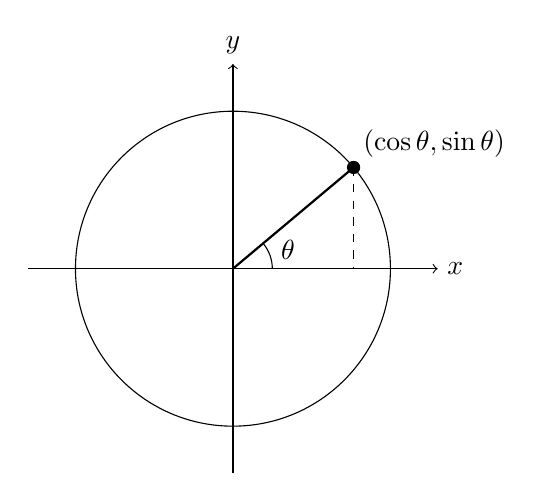
\begin{tikzpicture}[scale=2]
\draw[->] (-1.3,0)--(1.3,0) node[right] {\(x\)};
\draw[->] (0,-1.3)--(0,1.3) node[above] {\(y\)};
\draw (0,0) circle (1);
\draw[thick] (0,0)--({cos(40)},{sin(40)});
\draw[dashed] ({cos(40)},{sin(40)})--({cos(40)},0);
\fill ({cos(40)},{sin(40)}) circle (1.2pt);
\draw (0.25,0) arc[start angle=0,end angle=40,radius=0.25];
\node at (0.35,0.12) {\(\theta\)};
\node[above right] at ({cos(40)},{sin(40)})
{\((\cos\theta,\sin\theta)\)};
\end{tikzpicture}
\end{center}

This definition extends trigonometric functions beyond acute triangles.

%%%%%%%%%%%%%%%%%%%%%%%%%%%%%%%%%%%%%%%%%%%%%%%%%%%%%%%%%%%%
\subsection{Sine and Cosine}
\label{subsec:sine-cosine-functions}
%%%%%%%%%%%%%%%%%%%%%%%%%%%%%%%%%%%%%%%%%%%%%%%%%%%%%%%%%%%%

On the unit circle,

\[ \cos\theta=x, \]

and

\[ \sin\theta=y. \]

Because points on the unit circle satisfy

\[ x^2+y^2=1, \]

we obtain the fundamental identity

\[ \boxed{\sin^2\theta+\cos^2\theta=1.} \]

Here,

\[ \sin^2\theta \]

means

\[ (\sin\theta)^2. \]

%%%%%%%%%%%%%%%%%%%%%%%%%%%%%%%%%%%%%%%%%%%%%%%%%%%%%%%%%%%%
\subsection{The Other Trigonometric Functions}
\label{subsec:other-trigonometric-functions}
%%%%%%%%%%%%%%%%%%%%%%%%%%%%%%%%%%%%%%%%%%%%%%%%%%%%%%%%%%%%

The remaining standard trigonometric functions are defined using sine and
cosine:

\[ \tan\theta=\frac{\sin\theta}{\cos\theta}, \]

\[ \cot\theta=\frac{\cos\theta}{\sin\theta}, \]

\[ \sec\theta=\frac1{\cos\theta}, \]

and

\[ \csc\theta=\frac1{\sin\theta}. \]

They are read:

\begin{itemize}
    \item tangent;
    \item cotangent;
    \item secant;
    \item cosecant.
\end{itemize}

Each ratio is defined only when its denominator is nonzero.

%%%%%%%%%%%%%%%%%%%%%%%%%%%%%%%%%%%%%%%%%%%%%%%%%%%%%%%%%%%%
\subsection{Reference Angles and Quadrants}
\label{subsec:reference-angles-quadrants}
%%%%%%%%%%%%%%%%%%%%%%%%%%%%%%%%%%%%%%%%%%%%%%%%%%%%%%%%%%%%

The signs of sine and cosine depend on the quadrant.

\begin{center}
\begin{tikzpicture}[scale=1.4]
\draw[->] (-2.2,0)--(2.2,0);
\draw[->] (0,-2.2)--(0,2.2);

\node at (1.2,1.3) {I};
\node at (-1.2,1.3) {II};
\node at (-1.2,-1.3) {III};
\node at (1.2,-1.3) {IV};

\node[align=center] at (1.2,0.8) {\(\sin+\)\\\(\cos+\)};
\node[align=center] at (-1.2,0.8) {\(\sin+\)\\\(\cos-\)};
\node[align=center] at (-1.2,-0.8) {\(\sin-\)\\\(\cos-\)};
\node[align=center] at (1.2,-0.8) {\(\sin-\)\\\(\cos+\)};
\end{tikzpicture}
\end{center}

A reference angle is the acute angle between the terminal side of an angle
and the \(x\)-axis.

Reference angles allow trigonometric values throughout the plane to be
related to first-quadrant values.

%%%%%%%%%%%%%%%%%%%%%%%%%%%%%%%%%%%%%%%%%%%%%%%%%%%%%%%%%%%%
\subsection{Special-Angle Values}
\label{subsec:special-angle-values}
%%%%%%%%%%%%%%%%%%%%%%%%%%%%%%%%%%%%%%%%%%%%%%%%%%%%%%%%%%%%

Important unit-circle values include

\begin{center}
\begin{tabular}{c|cc}
\toprule
\(\theta\) & \(\cos\theta\) & \(\sin\theta\)\\
\midrule
\(0\) & \(1\) & \(0\)\\
\(\pi/6\) & \(\sqrt3/2\) & \(1/2\)\\
\(\pi/4\) & \(\sqrt2/2\) & \(\sqrt2/2\)\\
\(\pi/3\) & \(1/2\) & \(\sqrt3/2\)\\
\(\pi/2\) & \(0\) & \(1\)\\
\bottomrule
\end{tabular}
\end{center}

Symmetry and reference angles determine corresponding values in other
quadrants.

%%%%%%%%%%%%%%%%%%%%%%%%%%%%%%%%%%%%%%%%%%%%%%%%%%%%%%%%%%%%
\subsection{Periodic Functions}
\label{subsec:periodic-functions}
%%%%%%%%%%%%%%%%%%%%%%%%%%%%%%%%%%%%%%%%%%%%%%%%%%%%%%%%%%%%

\begin{definitionbox}{Periodic Function}
A function \(f\) is \emph{periodic} if there exists \(T>0\) such that
\[ f(x+T)=f(x) \]
for every applicable \(x\).
\end{definitionbox}

The smallest positive such \(T\), when it exists, is called the fundamental
period.

For sine and cosine,

\[ \sin(x+2\pi)=\sin x, \]

\[ \cos(x+2\pi)=\cos x. \]

Thus their fundamental period is

\[ 2\pi. \]

%%%%%%%%%%%%%%%%%%%%%%%%%%%%%%%%%%%%%%%%%%%%%%%%%%%%%%%%%%%%
\subsection{The Sine Function}
\label{subsec:sine-function-graph}
%%%%%%%%%%%%%%%%%%%%%%%%%%%%%%%%%%%%%%%%%%%%%%%%%%%%%%%%%%%%

The graph of

\[ y=\sin x \]

oscillates between \(-1\) and \(1\).

\begin{center}
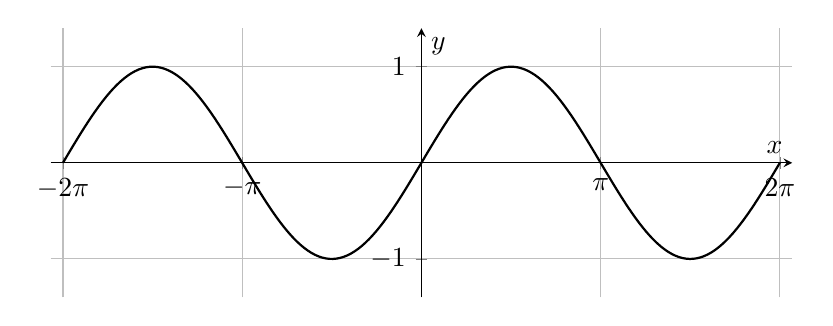
\begin{tikzpicture}
\begin{axis}[
    width=11cm,
    height=5cm,
    axis lines=middle,
    xmin=-6.5,xmax=6.5,
    ymin=-1.4,ymax=1.4,
    xlabel={$x$},
    ylabel={$y$},
    xtick={-6.283,-3.142,0,3.142,6.283},
    xticklabels={$-2\pi$,$-\pi$,$0$,$\pi$,$2\pi$},
    ytick={-1,0,1},
    samples=200,
    grid=major
]
\addplot[domain=-6.283:6.283,thick] {sin(deg(x))};
\end{axis}
\end{tikzpicture}
\end{center}

Its domain is

\[ \R, \]

and its range is

\[ [-1,1]. \]

%%%%%%%%%%%%%%%%%%%%%%%%%%%%%%%%%%%%%%%%%%%%%%%%%%%%%%%%%%%%
\subsection{The Cosine Function}
\label{subsec:cosine-function-graph}
%%%%%%%%%%%%%%%%%%%%%%%%%%%%%%%%%%%%%%%%%%%%%%%%%%%%%%%%%%%%

The graph of

\[ y=\cos x \]

has the same amplitude and period as sine but is horizontally shifted.

\begin{center}
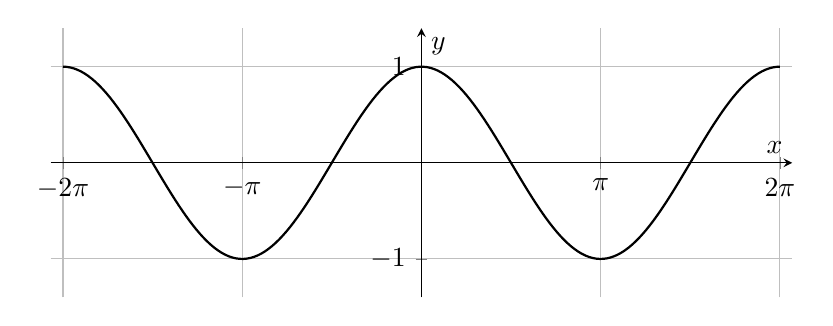
\begin{tikzpicture}
\begin{axis}[
    width=11cm,
    height=5cm,
    axis lines=middle,
    xmin=-6.5,xmax=6.5,
    ymin=-1.4,ymax=1.4,
    xlabel={$x$},
    ylabel={$y$},
    xtick={-6.283,-3.142,0,3.142,6.283},
    xticklabels={$-2\pi$,$-\pi$,$0$,$\pi$,$2\pi$},
    ytick={-1,0,1},
    samples=200,
    grid=major
]
\addplot[domain=-6.283:6.283,thick] {cos(deg(x))};
\end{axis}
\end{tikzpicture}
\end{center}

The domain is

\[ \R, \]

and the range is

\[ [-1,1]. \]

%%%%%%%%%%%%%%%%%%%%%%%%%%%%%%%%%%%%%%%%%%%%%%%%%%%%%%%%%%%%
\subsection{Amplitude, Period, Phase Shift, and Midline}
\label{subsec:sinusoidal-transformations}
%%%%%%%%%%%%%%%%%%%%%%%%%%%%%%%%%%%%%%%%%%%%%%%%%%%%%%%%%%%%

A transformed sinusoidal function often has the form

\[ y=A\sin(B(x-C))+D \]

or

\[ y=A\cos(B(x-C))+D. \]

When \(A\neq0\) and \(B\neq0\):

\[ \text{amplitude}=|A|, \]

\[ \text{period}=\frac{2\pi}{|B|}, \]

\[ \text{phase shift}=C, \]

and

\[ \text{midline}: y=D. \]

If \(A<0\), the graph is reflected across its midline.

%%%%%%%%%%%%%%%%%%%%%%%%%%%%%%%%%%%%%%%%%%%%%%%%%%%%%%%%%%%%
\subsection{Worked Example: Sinusoidal Features}
\label{subsec:worked-sinusoidal}
%%%%%%%%%%%%%%%%%%%%%%%%%%%%%%%%%%%%%%%%%%%%%%%%%%%%%%%%%%%%

\begin{workedexamplebox}{Analyzing a Sine Function}

Analyze

\[ y=-3\sin\left(2\left(x-\frac{\pi}{4}\right)\right)+1. \]

\begin{tabularx}{\textwidth}{@{}>{\raggedright\arraybackslash}p{0.42\textwidth}X@{}}
Identify \(A=-3\). &
Amplitude \(=3\); reflection across the midline.\\
Identify \(B=2\). &
Period \(=\dfrac{2\pi}{2}=\pi\).\\
Identify \(C=\pi/4\). &
Phase shift \(=\pi/4\) right.\\
Identify \(D=1\). &
Midline \(y=1\).
\end{tabularx}

\begin{answerbox}
\[
\boxed{
\text{Amplitude }3,\quad
\text{period }\pi,\quad
\text{shift right }\frac{\pi}{4},\quad
\text{midline }y=1.}
\]
\end{answerbox}
\end{workedexamplebox}

%%%%%%%%%%%%%%%%%%%%%%%%%%%%%%%%%%%%%%%%%%%%%%%%%%%%%%%%%%%%
\subsection{The Tangent Function}
\label{subsec:tangent-function-analysis}
%%%%%%%%%%%%%%%%%%%%%%%%%%%%%%%%%%%%%%%%%%%%%%%%%%%%%%%%%%%%

Because

\[ \tan x=\frac{\sin x}{\cos x}, \]

tangent is undefined wherever

\[ \cos x=0. \]

Thus vertical asymptotes occur at

\[ x=\frac{\pi}{2}+k\pi,\qquad k\in\Z. \]

Its fundamental period is

\[ \pi. \]

Its range is

\[ \R. \]

%%%%%%%%%%%%%%%%%%%%%%%%%%%%%%%%%%%%%%%%%%%%%%%%%%%%%%%%%%%%
\subsection{Transformed Tangent Functions}
\label{subsec:transformed-tangent}
%%%%%%%%%%%%%%%%%%%%%%%%%%%%%%%%%%%%%%%%%%%%%%%%%%%%%%%%%%%%

A tangent transformation often has the form

\[ y=A\tan(B(x-C))+D. \]

Its period is

\[ \frac{\pi}{|B|}. \]

The center point is

\[ (C,D). \]

Its neighboring vertical asymptotes are

\[ x=C-\frac{\pi}{2|B|} \]

and

\[ x=C+\frac{\pi}{2|B|}. \]

The line

\[ y=D \]

acts as its central horizontal reference or midline.

%%%%%%%%%%%%%%%%%%%%%%%%%%%%%%%%%%%%%%%%%%%%%%%%%%%%%%%%%%%%
\subsection{Fundamental Trigonometric Identities}
\label{subsec:fundamental-trig-identities}
%%%%%%%%%%%%%%%%%%%%%%%%%%%%%%%%%%%%%%%%%%%%%%%%%%%%%%%%%%%%

The Pythagorean identity is

\[ \sin^2x+\cos^2x=1. \]

Dividing by \(\cos^2x\), where defined, gives

\[ 1+\tan^2x=\sec^2x. \]

Dividing by \(\sin^2x\), where defined, gives

\[ 1+\cot^2x=\csc^2x. \]

Reciprocal identities include

\[ \sec x=\frac1{\cos x},\qquad
\csc x=\frac1{\sin x},\qquad
\cot x=\frac1{\tan x}. \]

%%%%%%%%%%%%%%%%%%%%%%%%%%%%%%%%%%%%%%%%%%%%%%%%%%%%%%%%%%%%
\subsection{Quotient Identities}
\label{subsec:quotient-identities}
%%%%%%%%%%%%%%%%%%%%%%%%%%%%%%%%%%%%%%%%%%%%%%%%%%%%%%%%%%%%

The quotient identities are

\[ \tan x=\frac{\sin x}{\cos x}, \]

and

\[ \cot x=\frac{\cos x}{\sin x}. \]

These identities allow many trigonometric expressions to be rewritten using
only sine and cosine.

%%%%%%%%%%%%%%%%%%%%%%%%%%%%%%%%%%%%%%%%%%%%%%%%%%%%%%%%%%%%
\subsection{Angle-Sum and Difference Identities}
\label{subsec:angle-sum-identities}
%%%%%%%%%%%%%%%%%%%%%%%%%%%%%%%%%%%%%%%%%%%%%%%%%%%%%%%%%%%%

For angles \(A\) and \(B\),

\[ \sin(A+B)=\sin A\cos B+\cos A\sin B, \]

\[ \sin(A-B)=\sin A\cos B-\cos A\sin B, \]

\[ \cos(A+B)=\cos A\cos B-\sin A\sin B, \]

and

\[ \cos(A-B)=\cos A\cos B+\sin A\sin B. \]

These identities produce double-angle, half-angle, and many other formulas.

%%%%%%%%%%%%%%%%%%%%%%%%%%%%%%%%%%%%%%%%%%%%%%%%%%%%%%%%%%%%
\subsection{Double-Angle Identities}
\label{subsec:double-angle-identities}
%%%%%%%%%%%%%%%%%%%%%%%%%%%%%%%%%%%%%%%%%%%%%%%%%%%%%%%%%%%%

Setting \(A=B=x\) gives

\[ \sin(2x)=2\sin x\cos x, \]

and

\[ \cos(2x)=\cos^2x-\sin^2x. \]

Equivalent cosine forms include

\[ \cos(2x)=2\cos^2x-1, \]

and

\[ \cos(2x)=1-2\sin^2x. \]

%%%%%%%%%%%%%%%%%%%%%%%%%%%%%%%%%%%%%%%%%%%%%%%%%%%%%%%%%%%%
\subsection{Inverse Trigonometric Functions}
\label{subsec:inverse-trigonometric-functions}
%%%%%%%%%%%%%%%%%%%%%%%%%%%%%%%%%%%%%%%%%%%%%%%%%%%%%%%%%%%%

Trigonometric functions are periodic and therefore not one-to-one over their
entire domains.

To define inverses, their domains must be restricted.

The principal inverse sine function is

\[ y=\arcsin x, \]

also written

\[ y=\sin^{-1}x. \]

It has domain

\[ [-1,1] \]

and range

\[ \left[-\frac{\pi}{2},\frac{\pi}{2}\right]. \]

The notation \(\sin^{-1}x\) means inverse sine, not \(1/\sin x\).

%%%%%%%%%%%%%%%%%%%%%%%%%%%%%%%%%%%%%%%%%%%%%%%%%%%%%%%%%%%%
\subsection{Inverse Cosine}
\label{subsec:inverse-cosine}
%%%%%%%%%%%%%%%%%%%%%%%%%%%%%%%%%%%%%%%%%%%%%%%%%%%%%%%%%%%%

The principal inverse cosine is

\[ y=\arccos x. \]

Its domain is

\[ [-1,1], \]

and its range is

\[ [0,\pi]. \]

Thus

\[ \arccos x=\theta \]

means

\[ \cos\theta=x \]

with

\[ 0\leq\theta\leq\pi. \]

%%%%%%%%%%%%%%%%%%%%%%%%%%%%%%%%%%%%%%%%%%%%%%%%%%%%%%%%%%%%
\subsection{Inverse Tangent}
\label{subsec:inverse-tangent}
%%%%%%%%%%%%%%%%%%%%%%%%%%%%%%%%%%%%%%%%%%%%%%%%%%%%%%%%%%%%

The principal inverse tangent is

\[ y=\arctan x. \]

Its domain is

\[ \R, \]

and its range is

\[ \left(-\frac{\pi}{2},\frac{\pi}{2}\right). \]

Thus

\[ \arctan x=\theta \]

means

\[ \tan\theta=x \]

with

\[ -\frac{\pi}{2}<\theta<\frac{\pi}{2}. \]

%%%%%%%%%%%%%%%%%%%%%%%%%%%%%%%%%%%%%%%%%%%%%%%%%%%%%%%%%%%%
\subsection{Average Rate of Change}
\label{subsec:average-rate-change}
%%%%%%%%%%%%%%%%%%%%%%%%%%%%%%%%%%%%%%%%%%%%%%%%%%%%%%%%%%%%

Suppose a function changes from \(f(a)\) to \(f(b)\).

The \emph{average rate of change} over \([a,b]\) is

\[ \frac{f(b)-f(a)}{b-a}. \]

This is exactly the slope of the secant line joining

\[ (a,f(a)) \]

and

\[ (b,f(b)). \]

\begin{center}
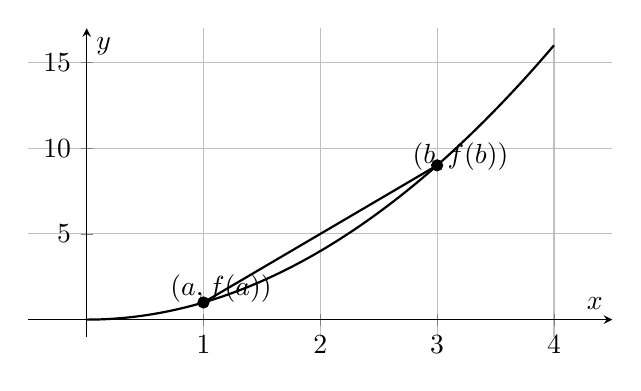
\begin{tikzpicture}
\begin{axis}[
    width=9cm,
    height=5.5cm,
    axis lines=middle,
    xmin=-0.5,xmax=4.5,
    ymin=-1,ymax=17,
    xlabel={$x$},
    ylabel={$y$},
    samples=100,
    grid=major
]
\addplot[domain=0:4,thick] {x^2};
\addplot[domain=1:3,thick] {4*x-3};
\addplot[only marks,mark=*] coordinates {(1,1) (3,9)};
\node at (axis cs:1.15,1.8) {$(a,f(a))$};
\node at (axis cs:3.2,9.5) {$(b,f(b))$};
\end{axis}
\end{tikzpicture}
\end{center}

%%%%%%%%%%%%%%%%%%%%%%%%%%%%%%%%%%%%%%%%%%%%%%%%%%%%%%%%%%%%
\subsection{The Difference Quotient}
\label{subsec:difference-quotient-precalc}
%%%%%%%%%%%%%%%%%%%%%%%%%%%%%%%%%%%%%%%%%%%%%%%%%%%%%%%%%%%%

If the second input is written

\[ x+h, \]

then the average rate of change from \(x\) to \(x+h\) is

\[ \frac{f(x+h)-f(x)}{h},\qquad h\neq0. \]

This expression is called the \emph{difference quotient}.

It is read:

``\(f\) of \(x+h\) minus \(f\) of \(x\), divided by \(h\).''

The difference quotient is the algebraic foundation of the derivative.

%%%%%%%%%%%%%%%%%%%%%%%%%%%%%%%%%%%%%%%%%%%%%%%%%%%%%%%%%%%%
\subsection{Worked Example: Difference Quotient}
\label{subsec:worked-difference-quotient}
%%%%%%%%%%%%%%%%%%%%%%%%%%%%%%%%%%%%%%%%%%%%%%%%%%%%%%%%%%%%

\begin{workedexamplebox}{Simplifying a Difference Quotient}

Let

\[ f(x)=x^2. \]

Simplify

\[ \frac{f(x+h)-f(x)}{h}. \]

\begin{tabularx}{\textwidth}{@{}>{\raggedright\arraybackslash}p{0.42\textwidth}X@{}}
Evaluate \(f(x+h)\). &
\(f(x+h)=(x+h)^2\)\\
Substitute into the quotient. &
\(\dfrac{(x+h)^2-x^2}{h}\)\\
Expand. &
\(\dfrac{x^2+2xh+h^2-x^2}{h}\)\\
Factor the numerator. &
\(\dfrac{h(2x+h)}{h}\)\\
Cancel \(h\), using \(h\neq0\). &
\(2x+h\)
\end{tabularx}

\begin{answerbox}
\[ \boxed{\frac{f(x+h)-f(x)}{h}=2x+h,\qquad h\neq0.} \]
\end{answerbox}
\end{workedexamplebox}

%%%%%%%%%%%%%%%%%%%%%%%%%%%%%%%%%%%%%%%%%%%%%%%%%%%%%%%%%%%%
\subsection{From Secant Lines to Tangent Lines}
\label{subsec:secant-to-tangent}
%%%%%%%%%%%%%%%%%%%%%%%%%%%%%%%%%%%%%%%%%%%%%%%%%%%%%%%%%%%%

The average rate of change gives the slope of a secant line.

Calculus asks what happens as the second point moves toward the first.

Symbolically, one studies what happens as

\[ h\to0. \]

The arrow

\[ \to \]

is read ``approaches'' in this context.

Thus

\[ h\to0 \]

is read ``\(h\) approaches zero.''

The limiting value of the difference quotient, when it exists, becomes the
instantaneous rate of change or derivative.

This transition is one of the central ideas of calculus.

%%%%%%%%%%%%%%%%%%%%%%%%%%%%%%%%%%%%%%%%%%%%%%%%%%%%%%%%%%%%
\subsection{Function Models}
\label{subsec:function-models}
%%%%%%%%%%%%%%%%%%%%%%%%%%%%%%%%%%%%%%%%%%%%%%%%%%%%%%%%%%%%

A mathematical model uses functions to represent relationships among
quantities.

Different models are appropriate for different patterns.

\begin{center}
\begin{tabularx}{0.92\textwidth}{@{}lX@{}}
\toprule
\textbf{Model} & \textbf{Typical Behavior}\\
\midrule
Linear & constant rate of change\\
Quadratic & acceleration or curved growth\\
Polynomial & flexible smooth algebraic behavior\\
Rational & ratios, saturation, reciprocal behavior\\
Exponential & constant proportional growth or decay\\
Logarithmic & inverse exponential behavior\\
Trigonometric & periodic or oscillatory behavior\\
Piecewise & behavior changing between regimes\\
\bottomrule
\end{tabularx}
\end{center}

Choosing an appropriate model requires both mathematical analysis and
knowledge of the context.

%%%%%%%%%%%%%%%%%%%%%%%%%%%%%%%%%%%%%%%%%%%%%%%%%%%%%%%%%%%%
\subsection{Linear Versus Exponential Growth}
\label{subsec:linear-exponential-growth}
%%%%%%%%%%%%%%%%%%%%%%%%%%%%%%%%%%%%%%%%%%%%%%%%%%%%%%%%%%%%

Linear growth adds approximately the same amount over equal intervals.

For example,

\[ P(t)=P_0+kt. \]

Exponential growth multiplies by approximately the same factor over equal
intervals.

For example,

\[ P(t)=P_0a^t. \]

This distinction is fundamental.

\begin{center}
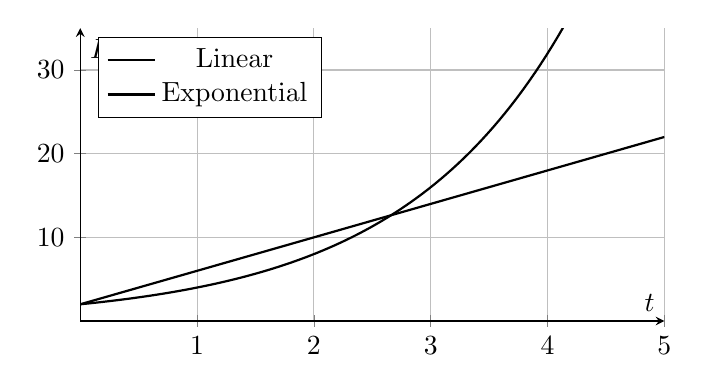
\begin{tikzpicture}
\begin{axis}[
    width=9cm,
    height=5.3cm,
    axis lines=middle,
    xmin=0,xmax=5,
    ymin=0,ymax=35,
    xlabel={$t$},
    ylabel={$P(t)$},
    samples=100,
    grid=major,
    legend pos=north west
]
\addplot[domain=0:5,thick] {2+4*x};
\addlegendentry{Linear}
\addplot[domain=0:5,thick] {2*2^x};
\addlegendentry{Exponential}
\end{axis}
\end{tikzpicture}
\end{center}

%%%%%%%%%%%%%%%%%%%%%%%%%%%%%%%%%%%%%%%%%%%%%%%%%%%%%%%%%%%%
\subsection{Asymptotic Behavior}
\label{subsec:precalculus-asymptotic-behavior}
%%%%%%%%%%%%%%%%%%%%%%%%%%%%%%%%%%%%%%%%%%%%%%%%%%%%%%%%%%%%

The word \emph{asymptotic} describes long-term or near-boundary behavior.

Questions include:

\begin{itemize}
    \item What happens as \(x\) becomes very large?
    \item What happens as \(x\) becomes very negative?
    \item What happens as \(x\) approaches a forbidden input?
    \item Does the function approach a finite value?
    \item Does the function grow without bound?
\end{itemize}

For example,

\[ f(x)=\frac{x}{x+1}. \]

Dividing numerator and denominator by \(x\),

\[ f(x)=\frac{1}{1+\frac1x}. \]

For very large \(|x|\), the term \(1/x\) becomes small, suggesting

\[ f(x)\approx1. \]

Thus

\[ y=1 \]

is a horizontal asymptote.

Formalizing this reasoning requires limits.

%%%%%%%%%%%%%%%%%%%%%%%%%%%%%%%%%%%%%%%%%%%%%%%%%%%%%%%%%%%%
\subsection{Functions and Units}
\label{subsec:functions-units}
%%%%%%%%%%%%%%%%%%%%%%%%%%%%%%%%%%%%%%%%%%%%%%%%%%%%%%%%%%%%

In applications, quantities often carry physical units.

Suppose

\[ d(t)=60t, \]

where \(d\) is measured in miles and \(t\) in hours.

Then the coefficient \(60\) has units

\[ \frac{\text{miles}}{\text{hour}}. \]

Rates of change therefore carry units of

\[ \frac{\text{output units}}{\text{input units}}. \]

Dimensional consistency provides an important way to detect errors in
applied mathematics.

%%%%%%%%%%%%%%%%%%%%%%%%%%%%%%%%%%%%%%%%%%%%%%%%%%%%%%%%%%%%
\subsection{Common Errors}
\label{subsec:precalculus-common-errors}
%%%%%%%%%%%%%%%%%%%%%%%%%%%%%%%%%%%%%%%%%%%%%%%%%%%%%%%%%%%%

\subsubsection{Confusing \(f(x)\) with Multiplication}

The notation

\[ f(x) \]

means the value of function \(f\) at \(x\).

It does not mean

\[ f\cdot x. \]

%%%%%%%%%%%%%%%%%%%%%%%%%%%%%%%%%%%%%%%%%%%%%%%%%%%%%%%%%%%%
\subsubsection{Ignoring Domain Restrictions}

An algebraic expression may be manipulable symbolically even when certain
inputs are excluded from the original function.

For example,

\[ \frac{(x-1)(x+1)}{x-1}=x+1 \]

only when

\[ x\neq1. \]

%%%%%%%%%%%%%%%%%%%%%%%%%%%%%%%%%%%%%%%%%%%%%%%%%%%%%%%%%%%%
\subsubsection{Confusing Domain and Range}

The domain consists of inputs.

The range consists of outputs.

%%%%%%%%%%%%%%%%%%%%%%%%%%%%%%%%%%%%%%%%%%%%%%%%%%%%%%%%%%%%
\subsubsection{Misreading Horizontal Shifts}

In

\[ f(x-C), \]

positive \(C\) shifts the graph right, not left.

%%%%%%%%%%%%%%%%%%%%%%%%%%%%%%%%%%%%%%%%%%%%%%%%%%%%%%%%%%%%
\subsubsection{Forgetting Reciprocal Horizontal Scaling}

In

\[ f(Bx), \]

the horizontal scale factor is

\[ \frac1{|B|}, \]

not \(|B|\).

%%%%%%%%%%%%%%%%%%%%%%%%%%%%%%%%%%%%%%%%%%%%%%%%%%%%%%%%%%%%
\subsubsection{Confusing \(f^{-1}\) with a Reciprocal}

The notation

\[ f^{-1}(x) \]

means inverse function.

The reciprocal is

\[ \frac1{f(x)}. \]

These are different constructions.

%%%%%%%%%%%%%%%%%%%%%%%%%%%%%%%%%%%%%%%%%%%%%%%%%%%%%%%%%%%%
\subsubsection{Assuming Every Function Has an Inverse Function}

An inverse function exists on the corresponding range only when the
function is one-to-one, or when its domain is suitably restricted.

%%%%%%%%%%%%%%%%%%%%%%%%%%%%%%%%%%%%%%%%%%%%%%%%%%%%%%%%%%%%
\subsubsection{Confusing Exponential and Power Functions}

In

\[ x^3, \]

the variable is the base.

In

\[ 3^x, \]

the variable is the exponent.

These functions behave very differently.

%%%%%%%%%%%%%%%%%%%%%%%%%%%%%%%%%%%%%%%%%%%%%%%%%%%%%%%%%%%%
\subsubsection{Applying Logarithm Laws to Sums}

In general,

\[ \log(x+y)\neq\log x+\log y. \]

Logarithm laws apply to products, quotients, and powers.

%%%%%%%%%%%%%%%%%%%%%%%%%%%%%%%%%%%%%%%%%%%%%%%%%%%%%%%%%%%%
\subsubsection{Using Degrees in Calculus Formulas}

Many calculus formulas for trigonometric functions assume angles are measured
in radians.

For example, the standard derivatives

\[ \dv{}{x}\sin x=\cos x \]

and

\[ \dv{}{x}\cos x=-\sin x \]

take this simple form when \(x\) is measured in radians.

%%%%%%%%%%%%%%%%%%%%%%%%%%%%%%%%%%%%%%%%%%%%%%%%%%%%%%%%%%%%
\subsubsection{Confusing \(\sin^{-1}x\) with \(\csc x\)}

The notation

\[ \sin^{-1}x \]

usually means inverse sine:

\[ \arcsin x. \]

The reciprocal of sine is

\[ \csc x=\frac1{\sin x}. \]

%%%%%%%%%%%%%%%%%%%%%%%%%%%%%%%%%%%%%%%%%%%%%%%%%%%%%%%%%%%%
\subsubsection{Confusing Average and Instantaneous Rate of Change}

The quantity

\[ \frac{f(b)-f(a)}{b-a} \]

is an average rate of change over an interval.

Instantaneous rate of change requires a limiting process.

%%%%%%%%%%%%%%%%%%%%%%%%%%%%%%%%%%%%%%%%%%%%%%%%%%%%%%%%%%%%
\subsection{Applications}
\label{subsec:precalculus-applications}
%%%%%%%%%%%%%%%%%%%%%%%%%%%%%%%%%%%%%%%%%%%%%%%%%%%%%%%%%%%%

\begin{applicationbox}
\textbf{Physics.}
Functions model position, velocity, acceleration, energy, waves, and
oscillations.

\medskip

\textbf{Biology.}
Exponential and logistic-type functions model populations, growth, decay,
and biological processes.

\medskip

\textbf{Economics.}
Functions describe cost, revenue, profit, supply, demand, and marginal
quantities.

\medskip

\textbf{Engineering.}
Trigonometric functions model periodic signals, rotations, vibrations, and
alternating currents.

\medskip

\textbf{Statistics.}
Probability distributions and statistical models are functions whose
properties are studied using calculus and analysis.

\medskip

\textbf{Differential Equations.}
Solutions of differential equations are functions whose rates of change
satisfy specified relationships.

\medskip

\textbf{Numerical Mathematics.}
Approximation, root finding, interpolation, and optimization require detailed
knowledge of function behavior.

\medskip

\textbf{Analysis.}
The concepts of domain, range, monotonicity, boundedness, inverse functions,
and asymptotic behavior become formal tools in real and complex analysis.
\end{applicationbox}

%%%%%%%%%%%%%%%%%%%%%%%%%%%%%%%%%%%%%%%%%%%%%%%%%%%%%%%%%%%%
\subsection{Exercises}
\label{subsec:precalculus-exercises}
%%%%%%%%%%%%%%%%%%%%%%%%%%%%%%%%%%%%%%%%%%%%%%%%%%%%%%%%%%%%

\begin{exercise}[1]
Let
\[ f(x)=3x^2-2x+5. \]
Compute \(f(0)\), \(f(2)\), and \(f(-1)\).
\end{exercise}

\begin{exercise}[2]
For
\[ f(x)=x^2+4x-3, \]
simplify \(f(x+h)\).
\end{exercise}

\begin{exercise}[2]
For
\[ f(x)=x^2+4x-3, \]
simplify
\[ \frac{f(x+h)-f(x)}{h}. \]
\end{exercise}

\begin{exercise}[1]
Find the domain of
\[ f(x)=\frac{1}{x+5}. \]
\end{exercise}

\begin{exercise}[2]
Find the domain of
\[ f(x)=\frac{\sqrt{2x-1}}{x-4}. \]
\end{exercise}

\begin{exercise}[2]
Find the domain of
\[ f(x)=\ln(7-x). \]
\end{exercise}

\begin{exercise}[1]
Find the range of
\[ f(x)=x^2+3. \]
\end{exercise}

\begin{exercise}[2]
Find the \(x\)- and \(y\)-intercepts of
\[ f(x)=x^2-5x+6. \]
\end{exercise}

\begin{exercise}[1]
Determine whether
\[ f(x)=x^4+2 \]
is even, odd, or neither.
\end{exercise}

\begin{exercise}[1]
Determine whether
\[ f(x)=x^5-3x \]
is even, odd, or neither.
\end{exercise}

\begin{exercise}[2]
Describe the transformations from \(y=x^2\) to
\[ y=3(x+2)^2-5. \]
\end{exercise}

\begin{exercise}[2]
Describe the transformations from \(y=|x|\) to
\[ y=-\frac12|x-4|+3. \]
\end{exercise}

\begin{exercise}[1]
Let
\[ f(x)=x+1,\qquad g(x)=x^2. \]
Find \(f+g\), \(fg\), \(f\circ g\), and \(g\circ f\).
\end{exercise}

\begin{exercise}[2]
Find the inverse of
\[ f(x)=5x+7. \]
\end{exercise}

\begin{exercise}[2]
Explain why
\[ f(x)=x^2 \]
does not have an inverse on all of \(\R\).
\end{exercise}

\begin{exercise}[2]
Restrict the domain of
\[ f(x)=x^2 \]
so that an inverse exists, and find that inverse.
\end{exercise}

\begin{exercise}[1]
Find the zeros of
\[ P(x)=x^2-9. \]
\end{exercise}

\begin{exercise}[2]
Factor
\[ P(x)=x^3-4x \]
and identify all zeros and multiplicities.
\end{exercise}

\begin{exercise}[2]
Describe the end behavior of
\[ P(x)=-3x^5+2x^2-7. \]
\end{exercise}

\begin{exercise}[2]
Find the vertical asymptotes of
\[ f(x)=\frac{x+2}{x^2-9}. \]
\end{exercise}

\begin{exercise}[2]
Determine whether
\[ f(x)=\frac{x^2-4}{x-2} \]
has a vertical asymptote or a hole at \(x=2\).
\end{exercise}

\begin{exercise}[1]
Find the domain and range of
\[ f(x)=\sqrt{x-3}. \]
\end{exercise}

\begin{exercise}[2]
Rewrite
\[ |x-4|<3 \]
as a compound inequality.
\end{exercise}

\begin{exercise}[1]
Evaluate
\[ \floor{4.8},\qquad \floor{-2.1}. \]
\end{exercise}

\begin{exercise}[1]
Classify
\[ f(x)=4^x \]
as exponential growth or decay.
\end{exercise}

\begin{exercise}[1]
Classify
\[ f(x)=\left(\frac13\right)^x \]
as exponential growth or decay.
\end{exercise}

\begin{exercise}[2]
Solve
\[ 3e^{2x}=20. \]
\end{exercise}

\begin{exercise}[2]
Solve
\[ 2^{x+1}=7. \]
\end{exercise}

\begin{exercise}[1]
Rewrite
\[ \log_2 32=5 \]
in exponential form.
\end{exercise}

\begin{exercise}[1]
Rewrite
\[ 10^3=1000 \]
in logarithmic form.
\end{exercise}

\begin{exercise}[2]
Expand
\[ \ln\left(\frac{x^3\sqrt y}{z}\right) \]
assuming all variables are positive.
\end{exercise}

\begin{exercise}[2]
Condense
\[ 2\ln x+\ln y-\ln z \]
into one logarithm.
\end{exercise}

\begin{exercise}[1]
Convert
\[ 150^\circ \]
to radians.
\end{exercise}

\begin{exercise}[1]
Convert
\[ \frac{5\pi}{6} \]
to degrees.
\end{exercise}

\begin{exercise}[1]
Find
\[ \sin\frac{\pi}{6},\qquad
\cos\frac{\pi}{6},\qquad
\tan\frac{\pi}{6}. \]
\end{exercise}

\begin{exercise}[1]
Find
\[ \sin\frac{3\pi}{4},\qquad
\cos\frac{3\pi}{4}. \]
\end{exercise}

\begin{exercise}[2]
Determine the reference angle of
\[ \frac{5\pi}{6}. \]
\end{exercise}

\begin{exercise}[1]
State the fundamental period of \(\sin x\), \(\cos x\), and \(\tan x\).
\end{exercise}

\begin{exercise}[2]
For
\[ y=4\cos(3x-\pi)-2, \]
determine amplitude, period, phase shift, and midline.
\end{exercise}

\begin{exercise}[2]
For
\[ y=-2\tan\left(4\left(x-\frac{\pi}{8}\right)\right)+3, \]
determine the period, center point, and neighboring vertical asymptotes.
\end{exercise}

\begin{exercise}[1]
Verify
\[ 1+\tan^2x=\sec^2x \]
using the Pythagorean identity.
\end{exercise}

\begin{exercise}[2]
Use an angle-sum identity to find
\[ \sin\frac{5\pi}{12}. \]
\end{exercise}

\begin{exercise}[2]
Derive
\[ \cos(2x)=1-2\sin^2x \]
from
\[ \cos(2x)=\cos^2x-\sin^2x. \]
\end{exercise}

\begin{exercise}[1]
Evaluate
\[ \arcsin\left(\frac12\right). \]
\end{exercise}

\begin{exercise}[1]
Evaluate
\[ \arccos\left(-\frac12\right). \]
\end{exercise}

\begin{exercise}[1]
Evaluate
\[ \arctan(1). \]
\end{exercise}

\begin{exercise}[2]
Explain why
\[ \sin^{-1}x \]
does not mean
\[ \frac1{\sin x}. \]
\end{exercise}

\begin{exercise}[1]
Find the average rate of change of
\[ f(x)=x^2 \]
from \(x=2\) to \(x=5\).
\end{exercise}

\begin{exercise}[2]
Find the average rate of change of
\[ f(x)=\frac1x \]
from \(x=1\) to \(x=4\).
\end{exercise}

\begin{exercise}[2]
For
\[ f(x)=3x^2-2x, \]
simplify the difference quotient
\[ \frac{f(x+h)-f(x)}{h}. \]
\end{exercise}

\begin{exercise}[2]
Explain geometrically what the difference quotient represents.
\end{exercise}

\begin{exercise}[2]
Explain the difference between linear and exponential growth.
\end{exercise}

\begin{exercise}[2]
A quantity is modeled by
\[ P(t)=500e^{0.04t}. \]
Identify the initial value and continuous growth rate.
\end{exercise}

\begin{exercise}[2]
A radioactive quantity satisfies
\[ A(t)=A_0e^{-0.08t}. \]
Find its half-life.
\end{exercise}

\begin{exercise}[2]
Explain why
\[ f(x)=\frac{x}{x+1} \]
approaches \(1\) for large \(|x|\).
\end{exercise}

\begin{exercise}[3]
For
\[ f(x)=\frac{x^2-1}{x^2-x}, \]
factor the expression, determine the domain, identify holes and vertical
asymptotes, and describe the horizontal asymptotic behavior.
\end{exercise}

\begin{exercise}[3]
Construct a function satisfying all of the following:
\begin{itemize}
    \item domain \(\R\setminus\{2\}\);
    \item a vertical asymptote at \(x=2\);
    \item a horizontal asymptote at \(y=3\);
    \item \(y\)-intercept \(1\).
\end{itemize}
\end{exercise}

%%%%%%%%%%%%%%%%%%%%%%%%%%%%%%%%%%%%%%%%%%%%%%%%%%%%%%%%%%%%
\subsection{Transition to Calculus}
\label{subsec:transition-to-calculus}
%%%%%%%%%%%%%%%%%%%%%%%%%%%%%%%%%%%%%%%%%%%%%%%%%%%%%%%%%%%%

Precalculus studies functions primarily through exact algebraic formulas,
graphs, transformations, and finite changes.

Calculus introduces a new question:

\begin{quote}
What happens when the change in the input becomes arbitrarily small?
\end{quote}

The difference quotient

\[ \frac{f(x+h)-f(x)}{h} \]

describes an average rate of change over a nonzero interval.

Calculus studies the behavior of this expression as

\[ h\to0. \]

Similarly, expressions such as

\[ f(x) \]

may be studied as

\[ x\to a. \]

The notation

\[ \lim_{x\to a}f(x) \]

is read:

``the limit of \(f(x)\) as \(x\) approaches \(a\).''

Here:

\begin{itemize}
    \item \(\lim\) means \emph{limit};
    \item \(x\to a\) means ``\(x\) approaches \(a\)'';
    \item the expression asks what value \(f(x)\) approaches as the input
    moves toward \(a\).
\end{itemize}

Limits provide the bridge from precalculus to calculus.

\begin{center}
\begin{tikzpicture}[
    node distance=10mm,
    box/.style={draw,rounded corners,align=center,inner sep=5pt},
    >=stealth
]
\node[box] (functions) {Functions};
\node[box,right=of functions] (rates) {Average rates\\of change};
\node[box,right=of rates] (limits) {Limits};
\node[box,right=of limits] (derivatives) {Derivatives};
\node[box,below=of limits] (integrals) {Integrals};
\node[box,below=of derivatives] (analysis) {Analysis};

\draw[->] (functions)--(rates);
\draw[->] (rates)--(limits);
\draw[->] (limits)--(derivatives);
\draw[->] (limits)--(integrals);
\draw[->] (derivatives)--(analysis);
\draw[->] (integrals)--(analysis);
\end{tikzpicture}
\end{center}

%%%%%%%%%%%%%%%%%%%%%%%%%%%%%%%%%%%%%%%%%%%%%%%%%%%%%%%%%%%%
\subsection{Section Connections}
\label{subsec:precalculus-connections}
%%%%%%%%%%%%%%%%%%%%%%%%%%%%%%%%%%%%%%%%%%%%%%%%%%%%%%%%%%%%

\chapterconnection{
Precalculus establishes the functional language required throughout
analysis. Functions are studied through their domains, ranges, graphs,
transformations, inverses, compositions, rates of change, asymptotes, and
long-term behavior. Polynomial, rational, radical, exponential, logarithmic,
trigonometric, inverse trigonometric, and piecewise-defined functions provide
the primary families used throughout elementary calculus. Radian measure and
the unit circle prepare trigonometric functions for differentiation and
integration, while exponential and logarithmic functions provide models of
growth and decay. The average rate of change and difference quotient lead
directly to the limiting processes that define derivatives. These ideas form
the transition from algebraic function analysis to the formal study of
limits, continuity, differentiation, and integration in
\cref{sec:single-variable-calculus}.
}

%%%%%%%%%%%%%%%%%%%%%%%%%%%%%%%%%%%%%%%%%%%%%%%%%%%%%%%%%%%%
% SECTION SOURCE TRACKING
%%%%%%%%%%%%%%%%%%%%%%%%%%%%%%%%%%%%%%%%%%%%%%%%%%%%%%%%%%%%

%------------------------------------------------------------
% 5.1 Precalculus and Functions
%------------------------------------------------------------
%
% Source:
%   - Lynn Marecek et al.,
%     Elementary Algebra.
%     Key: marecek2020elementaryalgebra
%
% Used for:
%   - algebraic function notation and evaluation;
%   - domain restrictions;
%   - polynomial and rational function foundations;
%   - transformations and algebraic manipulation;
%   - exponential and logarithmic foundations.
%
% Notes:
%   - The formal definition of a function is taught canonically in
%     Foundations.
%   - Elementary equation solving and polynomial algebra are taught
%     canonically in Elementary Algebra.
%   - Trigonometric material here is developed as the function-theoretic
%     preparation required for calculus rather than as a separate exhaustive
%     trigonometry course.
%   - Formal limit definitions belong to Single-Variable Calculus and Real
%     Analysis.
%   - Derivative and integral formulas are not developed here.
%   - More advanced asymptotic behavior belongs to Asymptotic Analysis.
%   - Visualizations and pedagogical organization are independently
%     developed for this text.
%
\nocite{marecek2020elementaryalgebra}